% !TeX spellcheck = pl_PL
%%%%%%%%%%%%%%%%%%%%%%%%%%%%%%%%%%%%%%%%%%%
%                                        %
% Szablon pracy dyplomowej inzynierskiej %
% zgodny  z aktualnymi  przepisami  SZJK %
%                                        %
%%%%%%%%%%%%%%%%%%%%%%%%%%%%%%%%%%%%%%%%%%
%                                        %
%  (c) Krzysztof Simiński, 2018-2023     %
%                                        %
%%%%%%%%%%%%%%%%%%%%%%%%%%%%%%%%%%%%%%%%%%
%                                        %
% Najnowsza wersja szablonów jest        %
% podstępna pod adresem                  %
% github.com/ksiminski/polsl-aei-theses  %
%                                        %
%%%%%%%%%%%%%%%%%%%%%%%%%%%%%%%%%%%%%%%%%%
%
%
% Projekt LaTeXowy zapewnia odpowiednie formatowanie pracy,
% zgodnie z wymaganiami Systemu zapewniania jakości kształcenia.
% Proszę nie zmieniać ustawień formatowania (np. fontu,
% marginesów, wytłuszczeń, kursywy itd. ).
%
% Projekt można kompilować na kilka sposobów.
%
% 1. kompilacja pdfLaTeX
%
% pdflatex main
% bibtex   main
% pdflatex main
% pdflatex main
%
%
% 2. kompilacja XeLaTeX
%
% Kompilatacja przy użyciu XeLaTeXa różni się tym, że na stronie
% tytułowej używany jest font Calibri. Wymaga to jego uprzedniego
% zainstalowania.
%
% xelatex main
% bibtex  main
% xelatex main
% xelatex main
%
%
%%%%%%%%%%%%%%%%%%%%%%%%%%%%%%%%%%%%%%%%%%%%%%%%%%%%%
% W przypadku pytań, uwag, proszę pisać na adres:   %
%      krzysztof.siminski(małpa)polsl.pl            %
%%%%%%%%%%%%%%%%%%%%%%%%%%%%%%%%%%%%%%%%%%%%%%%%%%%%%
%
% Chcemy ulepszać szablony LaTeXowe prac dyplomowych.
% Wypełniając ankietę spod poniższego adresu pomogą
% Państwo nam to zrobić. Ankieta jest całkowicie
% anonimowa. Dziękujemy!


% https://docs.google.com/forms/d/e/1FAIpQLScyllVxNKzKFHfILDfdbwC-jvT8YL0RSTFs-s27UGw9CKn-fQ/viewform?usp=sf_link
%
%%%%%%%%%%%%%%%%%%%%%%%%%%%%%%%%%%%%%%%%%%%%%%%%%%%%%%%%%%%%%%%%%%%%%%%%%

%%%%%%%%%%%%%%%%%%%%%%%%%%%%%%%%%%%%%%%%%%%%%%%
%                                             %
% PERSONALIZACJA PRACY – DANE PRACY           %
%                                             %
%%%%%%%%%%%%%%%%%%%%%%%%%%%%%%%%%%%%%%%%%%%%%%%

% Proszę wpisać swoje dane w poniższych definicjach.

%--------------------------------------
%
%
% TODO: None
%
% Status: 100% (DONE)
%--------------------------------------
% dane autora
\newcommand{\FirstNameAuthor}{Bartosz}
\newcommand{\SurnameAuthor}{Wuwer}
\newcommand{\IdAuthor}{296949}   % numer albumu  (bez $\langle$ i $\rangle$)

% drugi autor:
%\newcommand{\FirstNameCoauthor}{Imię}   % Jeżeli jest drugi autor, to tutaj należy podać imię.
%\newcommand{\SurnameCoauthor}{Nazwisko} % Jeżeli jest drugi autor, to tutaj należy podać nazwisko.
%\newcommand{\IdCoauthor}{$\langle$wpisać właściwy$\rangle$}  % numer albumu drugiego autora (bez $\langle$ i $\rangle$)
% Gdy nie ma drugiego autora, należy zostawić poniższe definicje puste, jak poniżej. Gdy jest drugi autor, należy zakomentować te linie.
\newcommand{\FirstNameCoauthor}{} % Jeżeli praca ma tylko jednego autora, to dane drugiego autora zostają puste.
\newcommand{\SurnameCoauthor}{}   % Jeżeli praca ma tylko jednego autora, to dane drugiego autora zostają puste.
\newcommand{\IdCoauthor}{}  % Jeżeli praca ma tylko jednego autora, to dane drugiego autora zostają puste.
%%%%%%%%%%

\newcommand{\Supervisor}{Dr inż. Krzysztof Jaskot}     % dane promotora (bez $\langle$ i $\rangle$)
\newcommand{\Title}{System wizyjny do śledzenia ruchu gałek ocznych}           % tytuł pracy po polsku
\newcommand{\TitleAlt}{Vision system for tracking the movement of the eyeballs}                     % thesis title in English
\newcommand{\Program}{Automatyka i Robotyka}            % kierunek studiów  (bez $\langle$ i $\rangle$)
\newcommand{\Specialisation}{Technologie informacyjne w automatyce i robotyce}     % specjalność  (bez $\langle$ i $\rangle$)
\newcommand{\Departament}{Automatyki i Robotyki}        % katedra promotora  (bez $\langle$ i $\rangle$)

% Jeżeli został wyznaczony promotor pomocniczy lub opiekun, proszę go/ją wpisać ...
\newcommand{\Consultant}{} % dane promotora pomocniczego, opiekuna (bez $\langle$ i $\rangle$)
% ... w przeciwnym razie proszę zostawić puste miejsce jak poniżej:
%\newcommand{\Consultant}{} % brak promotowa pomocniczego / opiekuna

% koniec fragmentu do modyfikacji
%%%%%%%%%%%%%%%%%%%%%%%%%%%%%%%%%%%%%%%%%%


%%%%%%%%%%%%%%%%%%%%%%%%%%%%%%%%%%%%%%%%%%%%%%%
%                                             %
% KONIEC PERSONALIZACJI PRACY                 %
%                                             %
%%%%%%%%%%%%%%%%%%%%%%%%%%%%%%%%%%%%%%%%%%%%%%%

%%%%%%%%%%%%%%%%%%%%%%%%%%%%%%%%%%%%%%%%


%%%%%%%%%%%%%%%%%%%%%%%%%%%%%%%%%%%%%%%%%%%%%%%
%                                             %
% PROSZĘ NIE MODYFIKOWAĆ PONIŻSZYCH USTAWIEŃ! %
%                                             %
%%%%%%%%%%%%%%%%%%%%%%%%%%%%%%%%%%%%%%%%%%%%%%%



\documentclass[a4paper,twoside,12pt]{book}
\usepackage[utf8]{inputenc}                                      
\usepackage[T1]{fontenc}  
\usepackage{amsmath,amsfonts,amssymb,amsthm}
\usepackage[british,polish]{babel} 
\usepackage{indentfirst}
\usepackage{xurl}
\usepackage{xstring}
\usepackage{ifthen}



\usepackage{ifxetex}

\ifxetex
	\usepackage{fontspec}
	\defaultfontfeatures{Mapping=tex—text} % to support TeX conventions like ``——-''
	\usepackage{xunicode} % Unicode support for LaTeX character names (accents, European chars, etc)
	\usepackage{xltxtra} % Extra customizations for XeLaTeX
\else
	\usepackage{lmodern}
\fi



\usepackage[margin=2.5cm]{geometry}
\usepackage{graphicx} 
\usepackage{hyperref}
\usepackage{booktabs}
\usepackage{tikz}
\usepackage{pgfplots}
\usepackage{mathtools}
\usepackage{geometry}
\usepackage{subcaption}   % subfigures
\usepackage[page]{appendix} % toc,
\renewcommand{\appendixtocname}{Dodatki}
\renewcommand{\appendixpagename}{Dodatki}
\renewcommand{\appendixname}{Dodatek}

\usepackage{csquotes}
\usepackage[natbib=true,backend=bibtex,maxbibnames=99]{biblatex}  % kompilacja bibliografii BibTeXem
%\usepackage[natbib=true,backend=biber,maxbibnames=99]{biblatex}  % kompilacja bibliografii Biberem
\bibliography{biblio}

\usepackage{ifmtarg}   % empty commands  

\usepackage{setspace}
\onehalfspacing


\frenchspacing



%%%% TODO LIST GENERATOR %%%%%%%%%

\usepackage{color}
\definecolor{brickred}      {cmyk}{0   , 0.89, 0.94, 0.28}

\makeatletter \newcommand \kslistofremarks{\section*{Uwagi} \@starttoc{rks}}
  \newcommand\l@uwagas[2]
    {\par\noindent \textbf{#2:} %\parbox{10cm}
{#1}\par} \makeatother


\newcommand{\ksremark}[1]{%
{%\marginpar{\textdbend}
{\color{brickred}{[#1]}}}%
\addcontentsline{rks}{uwagas}{\protect{#1}}%
}

\newcommand{\comma}{\ksremark{przecinek}}
\newcommand{\nocomma}{\ksremark{bez przecinka}}
\newcommand{\styl}{\ksremark{styl}}
\newcommand{\ortografia}{\ksremark{ortografia}}
\newcommand{\fleksja}{\ksremark{fleksja}}
\newcommand{\pauza}{\ksremark{pauza `--', nie dywiz `-'}}
\newcommand{\kolokwializm}{\ksremark{kolokwializm}}
\newcommand{\cudzyslowy}{\ksremark{,,polskie cudzysłowy''}}

%%%%%%%%%%%%%% END OF TODO LIST GENERATOR %%%%%%%%%%%

\newcommand{\printCoauthor}{%		
    \StrLen{\FirstNameCoauthor}[\FNCoALen]
    \ifthenelse{\FNCoALen > 0}%
    {%
		{\large\bfseries\Coauthor\par}
	
		{\normalsize\bfseries \LeftId: \IdCoauthor\par}
    }%
    {}
} 

%%%%%%%%%%%%%%%%%%%%%
\newcommand{\autor}{%		
    \StrLen{\FirstNameCoauthor}[\FNCoALenXX]
    \ifthenelse{\FNCoALenXX > 0}%
    {\FirstNameAuthor\ \SurnameAuthor, \FirstNameCoauthor\ \SurnameCoauthor}%
	{\FirstNameAuthor\ \SurnameAuthor}%
}
%%%%%%%%%%%%%%%%%%%%%

\StrLen{\FirstNameCoauthor}[\FNCoALen]
\ifthenelse{\FNCoALen > 0}%
{%
\author{\FirstNameAuthor\ \SurnameAuthor, \FirstNameCoauthor\ \SurnameCoauthor}
}%
{%
\author{\FirstNameAuthor\ \SurnameAuthor}
}%

%%%%%%%%%%%% ZYWA PAGINA %%%%%%%%%%%%%%%
% brak kapitalizacji zywej paginy
\usepackage{fancyhdr}
\pagestyle{fancy}
\fancyhf{}
\fancyhead[LO]{\nouppercase{\it\rightmark}}
\fancyhead[RE]{\nouppercase{\it\leftmark}}
\fancyhead[LE,RO]{\it\thepage}


\fancypagestyle{tylkoNumeryStron}{%
   \fancyhf{} 
   \fancyhead[LE,RO]{\it\thepage}
}

\fancypagestyle{bezNumeracji}{%
   \fancyhf{} 
   \fancyhead[LE,RO]{}
}


\fancypagestyle{NumeryStronNazwyRozdzialow}{%
   \fancyhf{} 
   \fancyhead[LE]{\nouppercase{\autor}}
   \fancyhead[RO]{\nouppercase{\leftmark}} 
   \fancyfoot[CE, CO]{\thepage}
}


%%%%%%%%%%%%% OBCE WTRETY  
\newcommand{\obcy}[1]{\emph{#1}}
\newcommand{\english}[1]{{\selectlanguage{british}\obcy{#1}}}
%%%%%%%%%%%%%%%%%%%%%%%%%%%%%

% polskie oznaczenia funkcji matematycznych
\renewcommand{\tan}{\operatorname {tg}}
\renewcommand{\log}{\operatorname {lg}}

% jeszcze jakies drobiazgi

\newcounter{stronyPozaNumeracja}

%%%%%%%%%%%%%%%%%%%%%%%%%%% 
\newcommand{\printOpiekun}[1]{%		

    \StrLen{\Consultant}[\mystringlen]
    \ifthenelse{\mystringlen > 0}%
    {%
       {\large{\bfseries OPIEKUN, PROMOTOR POMOCNICZY}\par}
       
       {\large{\bfseries \Consultant}\par}
    }%
    {}
} 
%
%%%%%%%%%%%%%%%%%%%%%%%%%%%%%%%%%%%%%%%%%%%%%%
 
% Proszę nie modyfikować poniższych definicji!
\newcommand{\Author}{\FirstNameAuthor\ \MakeUppercase{\SurnameAuthor}} 
\newcommand{\Coauthor}{\FirstNameCoauthor\ \MakeUppercase{\SurnameCoauthor}}
\newcommand{\Type}{PROJEKT INŻYNIERSKI}
\newcommand{\Faculty}{Wydział Automatyki, Elektroniki i Informatyki} 
\newcommand{\Polsl}{Politechnika Śląska}
\newcommand{\Logo}{politechnika_sl_logo_bw_pion_pl.pdf}
\newcommand{\LeftId}{Nr albumu}
\newcommand{\LeftProgram}{Kierunek}
\newcommand{\LeftSpecialisation}{Specjalność}
\newcommand{\LeftSUPERVISOR}{PROWADZĄCY PRACĘ}
\newcommand{\LeftDEPARTMENT}{KATEDRA}
%%%%%%%%%%%%%%%%%%%%%%%%%%%%%%%%%%%%%%%%%%%%%%

%%%%%%%%%%%%%%%%%%%%%%%%%%%%%%%%%%%%%%%%%%%%%%%
%                                             %
% KONIEC USTAWIEŃ                             %
%                                             %
%%%%%%%%%%%%%%%%%%%%%%%%%%%%%%%%%%%%%%%%%%%%%%%




%%%%%%%%%%%%%%%%%%%%%%%%%%%%%%%%%%%%%%%%%%%%%%%
%                                             %
% MOJE PAKIETY, USTAWIENIA ITD                %
%                                             %
%%%%%%%%%%%%%%%%%%%%%%%%%%%%%%%%%%%%%%%%%%%%%%%

% Tutaj proszę umieszczać swoje pakiety, makra, ustawienia itd.

\usepackage{siunitx}
\sisetup{locale = PL}

\usepackage{float}

\usepackage{placeins}
 
%%%%%%%%%%%%%%%%%%%%%%%%%%%%%%%%%%%%%%%%%%%%%%%%%%%%%%%%%%%%%%%%%%%%%
% listingi i fragmentu kodu źródłowego 
% pakiet: listings lub minted
% % % % % % % % % % % % % % % % % % % % % % % % % % % % % % % % % % % 

% biblioteka listings
\usepackage{listings}
\lstset{%
morekeywords={string,exception,std,vector},% słowa kluczowe rozpoznawane przez pakiet listings
language=Python,% C, Matlab, Python, SQL, TeX, XML, bash, ... – vide https://www.ctan.org/pkg/listings
commentstyle=\textit,%
identifierstyle=\textsf,%
keywordstyle=\sffamily\bfseries, %\texttt, %
%captionpos=b,%
tabsize=3,%
frame=lines,%
numbers=left,%
numberstyle=\tiny,%
numbersep=5pt,%
breaklines=true,%
escapeinside={@*}{*@},%
}

% % % % % % % % % % % % % % % % % % % % % % % % % % % % % % % % % % % 
% pakiet minted
%\usepackage{minted}

% pakiet wymaga specjalnego kompilowania:
% pdflatex -shell-escape main.tex
% xelatex  -shell-escape main.tex

%\usepackage[chapter]{minted} % [section]
%%\usemintedstyle{bw}   % czarno-białe kody 
%
%\setminted % https://ctan.org/pkg/minted
%{
%%fontsize=\normalsize,%\footnotesize,
%%captionpos=b,%
%tabsize=3,%
%frame=lines,%
%framesep=2mm,
%numbers=left,%
%numbersep=5pt,%
%breaklines=true,%
%escapeinside=@@,%
%}

%%%%%%%%%%%%%%%%%%%%%%%%%%%%%%%%%%%%%%%%%%%%%%%%%%%%%%%%%%%%%%%%%%%%%



%%%%%%%%%%%%%%%%%%%%%%%%%%%%%%%%%%%%%%%%%%%%%%%
%                                             %
% KONIEC MOICH USTAWIEŃ                       %
%                                             %
%%%%%%%%%%%%%%%%%%%%%%%%%%%%%%%%%%%%%%%%%%%%%%%



%%%%%%%%%%%%%%%%%%%%%%%%%%%%%%%%%%%%%%%%


\begin{document}
%\kslistofremarks

\frontmatter

%%%%%%%%%%%%%%%%%%%%%%%%%%%%%%%%%%%%%%%%%%%%%%%
%                                             %
% PROSZĘ NIE MODYFIKOWAĆ STRONY TYTUŁOWEJ!    %
%                                             %
%%%%%%%%%%%%%%%%%%%%%%%%%%%%%%%%%%%%%%%%%%%%%%%


%%%%%%%%%%%%%%%%%%  STRONA TYTUŁOWA %%%%%%%%%%%%%%%%%%%
\pagestyle{empty}
{
	\newgeometry{top=1.5cm,%
	             bottom=2.5cm,%
	             left=3cm,
	             right=2.5cm}
 
	\ifxetex 
	  \begingroup
	  \setsansfont{Calibri}
	   
	\fi 
	 \sffamily
	\begin{center}
	\includegraphics[width=50mm]{\Logo}
	 
	
	{\Large\bfseries\Type\par}
	
	\vfill  \vfill  
			 
	{\large\Title\par}
	
	\vfill  
		
	{\large\bfseries\Author\par}
	
	{\normalsize\bfseries \LeftId: \IdAuthor}

	\printCoauthor
	
	\vfill  		
 
	{\large{\bfseries \LeftProgram:} \Program\par} 
	
	{\large{\bfseries \LeftSpecialisation:} \Specialisation\par} 
	 		
	\vfill  \vfill 	\vfill 	\vfill 	\vfill 	\vfill 	\vfill  
	 
	{\large{\bfseries \LeftSUPERVISOR}\par}
	
	{\large{\bfseries \Supervisor}\par}
				
	{\large{\bfseries \LeftDEPARTMENT\ \Departament} \par}
		
	{\large{\bfseries \Faculty}\par}
		
	\vfill  \vfill  

    	
    \printOpiekun{\Consultant}
    
	\vfill  \vfill  
		
    {\large\bfseries  Gliwice \the\year}

   \end{center}	
       \ifxetex 
       	  \endgroup
       \fi
	\restoregeometry
}
  
%%%%%%%%%%%%%%%%%%%%%%%%%%%%%%%%%%%%%%%%%%%%%%%
%                                             %
% KONIEC STRONY TYTUŁOWEJ                     %
%                                             %
%%%%%%%%%%%%%%%%%%%%%%%%%%%%%%%%%%%%%%%%%%%%%%%  


\cleardoublepage

\rmfamily\normalfont
\pagestyle{empty}


%%% No to zaczynamy pisać pracę :-) %%%%

%--------------------------------------
%
%
% TODO: Streszczenie, słowa kluczowe, abstract, keywords
%
% Status: 0%
%--------------------------------------
\subsubsection*{Tytuł pracy} 
\Title

\subsubsection*{Streszczenie}  
(Streszczenie pracy – odpowiednie pole w systemie APD powinno zawierać kopię tego streszczenia.)

\subsubsection*{Słowa kluczowe} 
(2-5 slow (fraz) kluczowych, oddzielonych przecinkami)

\subsubsection*{Thesis title} 
\begin{otherlanguage}{british}
\TitleAlt
\end{otherlanguage}

\subsubsection*{Abstract} 
\begin{otherlanguage}{british}
(Thesis abstract – to be copied into an appropriate field during an electronic submission – in English.)
\end{otherlanguage}
\subsubsection*{Key words}  
\begin{otherlanguage}{british}
(2-5 keywords, separated by commas)
\end{otherlanguage}




%%%%%%%%%%%%%%%%%% SPIS TRESCI %%%%%%%%%%%%%%%%%%%%%%
% Add \thispagestyle{empty} to the toc file (main.toc), because \pagestyle{empty} doesn't work if the TOC has multiple pages
\addtocontents{toc}{\protect\thispagestyle{empty}}
\tableofcontents

%%%%%%%%%%%%%%%%%%%%%%%%%%%%%%%%%%%%%%%%%%%%%%%%%%%%%
\setcounter{stronyPozaNumeracja}{\value{page}}
\mainmatter
\pagestyle{empty}

\cleardoublepage

\pagestyle{NumeryStronNazwyRozdzialow}

%%%%%%%%%%%%%% wlasciwa tresc pracy %%%%%%%%%%%%%%%%%

%--------------------------------------
%
%
% TODO: cel pracy (99.9%), zakres pracy(99%), zwięzła charakterystyka rozdziałów
%
% Status: 80%
%--------------------------------------
\chapter{Wstęp}
\label{ch:wstep}

\section{Wprowadzenie i osadzenie w dziedzinie}
\label{sec:wprowadzenie-i-osadzenie-w-dziedzinie}
% wprowadzenie w problem/zagadnienie
Śledzenie ruchu gałek ocznych (ang. eye-tracking), zwane również jako okulografia, jest techniką, która badana jest od ponad stu lat. Istotność tej techniki wynika z faktu, że ruchy gałek ocznych są ściśle związane z procesami poznawczymi, takimi jak uwaga, percepcja, pamięć, czy procesy decyzyjne. Skupiając wzrok na danym punkcie, umieszczamy go w centralnym obszarze naszego pola widzenia które charakteryzuje się największą rozdzielczością, co pozwala na dokładne analizowanie szczegółów. Ten fakt wpływa także na proces skupienia -- gdy koncentrujemy się na danym obiekcie lub obszarze, skupiamy na nim wzrok (często wystarczy jedynie krótki moment).

Możliwość rejestrowania ruchów oczu pozwala na zrozumienie w jaki sposób obserwator eksploruje otaczający go świat. Posiadając tą wiedzę możliwe jest wyciągnięcie wniosków na temat tego co jest interesujące lub istotne dla obserwatora, jakie emocje się z tym wiążą, czy nawet jakie procesy poznawcze zachodzą w jego umyśle, czy rozumie on to co widzi. Nie trudnym jest zauważyć jak cenne mogą być te informacje w szerokim spektrum dziedzin.

% osadzenie problemu w dziedzinie
Okulografia odgrywa kluczową rolę w psychologi poznawczej, psychologi społecznej, neurobiologii, marketingu, czy medycynie. W psychologii poznawczej ruch oczu jest ściśle związany z pamięcią, podejmowaniem decyzji, obciążeniem poznawczym i uczeniem się asocjacyjnym. W psychologii społecznej eye-tracking pozwala na wgląd w zachowania społeczne i ich analizę, co pozwala badać empatię, prospołeczność, czy fobie społeczne \cite{bib:tobii-main}. W neurobiologii bada się powiązania ruchu oczu ze szlakami neuronowymi odpowiedzialnymi za podejmowane akcje i procesy myślowe, dając możliwość w diagnozach i wsparciu osób dotkniętych chorobą Parkinsona \cite{bib:tobii-parkinson}, Alzheimera \cite{bib:tobii-alzheimer}, a także autyzmem czy łagodnym upośledzeniem funkcji poznawczych \cite{bib:tobii-autyzm}. W medycynie okulografia pozwala na diagnozę między innymi oczopląsu, który może być objawem np. stwardnienia rozsianego, uszkodzenia śródmózgowia lub urazu ucha wewnętrznego \cite{bib:Diagnostyka-oczoplas}. Niezaprzeczalnie technika ta jest niezwykle cenna i efektywna na wielu płaszczyznach naukowych i praktycznych.

\section{Cel oraz zakres pracy}
\label{sec:cel-oraz-zakres-pracy}
% cel pracy
Celem niniejszej pracy jest wykonanie narzędzia które pozwoli na uniwersalne śledzenie ruchu gałek ocznych, bez zdefiniowanej docelowej grupy użytkowników. System ten powinien być prosty w obsłudze i niewymagający zaawansowanej technologii, ale nie ograniczający w razie potrzeby bardziej zaawansowanych użytkowników, prezentując użyteczność zarówno dla naukowców, studentów, jak i hobbystów. Tego typu narzędzie pozwoli na eksplorację danych eye-trackingowych, otwierając możliwości na dalszą analizę i interpretację wyników, a także zapewni solidną podstawę w razie potrzeby modyfikacji lub rozbudowy systemu w bardziej ukierunkowany sposób.

% zakres pracy
Praca ta skupia się przede wszystkim na samym procesie wykrywania źrenic i śledzenia ruchu gałek ocznych na ich podstawie oraz implementacji systemu wizyjnego, który pozwoli na zapis, wizualizację i potencjalną dalszą analizę danych zebranych przez kamerę, w tym także kamerę internetową. Całość zrealizowana jest w języku Python, z wykorzystaniem bibliotek takich jak OpenCV, NumPy, pandas oraz Matplotlib, a wszelkie prezentowane dane zostały uchwycone przy użyciu wbudowanej kamery laptopa. Praca nie będzie obejmować rozległej analizy zebranych danych, ani eksperymentów przeprowadzonych z użyciem owego systemu. Nie została także stworzona grupa testowa, więc większość testów przeprowadzone zostały na autorze pracy.

\begin{itemize}
\item wprowadzenie w problem/zagadnienie
\item osadzenie problemu w dziedzinie
\item cel pracy
\item zakres pracy
\item zwięzła charakterystyka rozdziałów
\item jednoznaczne określenie wkładu autora, w przypadku prac wieloosobowych – tabela z autorstwem poszczególnych elementów pracy
\end{itemize}



%--------------------------------------
%
%
% TODO: Dodać zdjęcia???, tytuł tematu???, krótkie wprowadzenie na początku każdej sekcji/rozdziału
%
% Status: 99.98%
%--------------------------------------
\chapter{Śledzenie ruchu gałek ocznych -- analiza tematu}
\label{ch:analiza-tematu}

\section{Sformułowanie problemu}
\label{sec:sformulowanie-problemu}

Widzeniem plamkowym (fovealnym) nazywamy wspomniane już wcześniej zjawisko, że widzimy w największej rozdzielczości jedynie centrum pola widzenia. Wynika to z budowy siatkówki, która posiada plamkę żółtą (fovea) -- jest to niewielki obszar, który charakteryzuje się największym zagęszczeniem czopków. Taka budowa siatkówki sprawia, że nieustannie poruszamy oczami. Skupiając wzrok na danym punkcie, musimy być gotowi na to, że cała reszta pola widzenia straci dla nas na ostrości. Jest to proces, który przypomina filtracje wielu otaczających nas informacji, do paru, które mają w tym momencie znaczenie.

\subsection{Uwaga wzrokowa}
\label{subsec:uwaga-wzrokowa}

Uwaga wzrokowa może zostać opisana przez idiomy ,,gdzie'' i ,,co'', które pozwalają na zobrazowanie jej selektywnej natury. ,,Gdzie'' to proces wizualnego wyszukiwania i wyboru lokalizacji, która zwróciła naszą uwagę, w celu dokładniejszego zbadania. Istotnym aspektem tego procesu selekcji jest widzenie peryferyjne, czyli takie obejmujące obszar oddalony od naszego punktu skupienia, ale wciąż pozwalający na wyodrębnienie kształtów i ruchu, co w pewien sposób prowadzi nasze centralne spojrzenie. Przykładem może być spojrzenie przez okno -- w pierwszym momencie nasz wzrok kierowany jest na wyraźne kształty, światła czy nagłe ruchy jak np. lądujący ptak. 

,,Co'' można nazwać odwrotnością ,,gdzie'' -- jest to proces szczegółowego badania danego obszaru, charakteryzują go takie zjawiska jak fiksacja, czyli stabilizacja wzroku na danym punkcie oraz ruchy sakadowe, czyli szybkie mimowolne ruchy oczu pomiędzy kolejnymi punktami, które pozwalają na obserwacje. Całość tworzy kanał percepcyjny o ograniczonym zasięgu przestrzennym, obejmujący interesujący obszar, budując w ten sposób naszą świadomość i zrozumienie celu naszego spojrzenia. Wracając do poprzedniego przykładu, po zauważeniu ptaka, nasze spojrzenie skupi się na nim (fiksacja), a ruchy sakadowe oczu pozwolą na dokładne zbadanie jego kształtu, koloru i detali. To właśnie połączenie ,,gdzie'' i ,,co'' pozwala na głębsze zrozumienie otaczającego nas świata, a owe ścieżki skanowania dają nam 
wgląd w proces poznawczy badanej osoby, jako że pomiar widzenia fovealnego w czasie odzwierciedla chwilowe i jawne skupienie uwagi wzrokowej obserwatora. 

\subsection{Poszukiwanie wzrokowe}
\label{subsec:poszukiwanie-wzrokowe}

Tutaj warto wspomnieć o poszukiwaniu wzrokowym, jest to proces aktywnego przeszukiwania pola widzenia w celu znalezienia konkretnego celu, a częścią tego procesu jest etap przeduwagowy. Etap ten równolegle analizuje duży obszar widzenia jednocześnie, dzieje się to automatycznie, nieświadomie i nie wymaga widzenia fovealnego. Co charakteryzuje ten proces to umiejętność rozpoznania czterech podstawowych cech: kolor, rozmiar, orientacja oraz obecność i/lub kierunek ruchu. Etap przeduwagowy jest pierwszym krokiem poszukiwania wzrokowego i obejmuje dużą część poszukiwania typu równoległego (np. próba zauważenia nagłego ruchu spadającej gwiazdy) i relatywnie niewielką część poszukiwania typu seryjnego (np. przeszukiwanie obiektów na stole w poszukiwaniu kluczy), które wymaga uwagi i przenoszenia wzroku od obiektu do obiektu. 

\subsection{Analiza ruchów oczu}
\label{subsec:analiza-ruchow-oczu}

Powyższe rozważania pozwalają przejść do głównego nurtu tematu śledzenia ruchu gałek ocznych, czyli analiza ruchów oczu. Rozróżniamy pięć podstawowych typów ruchów oczu: wspomniane już wcześniej sakadyczne, wergencyjne, przedsionkowe, płynne podążanie (smooth pursuit) oraz oczopląs fizjologiczny, który jest naturalny dla zdrowej osoby i często występuje podczas fiksacji. Ruchy te można podzielić na dobrowolne, mimowolne i odruchowe, a sygnały je kontrolujące pochodzą z obszarów korowych mózgu. Do opisania tych procesów można posłużyć się modelowaniem matematycznym. Do zrozumienia jawnej uwagi wzrokowej wystarczy modelowanie trzech typów ruchów: fiksacji, która pokazuje chęć utrzymania wzroku na stacjonarnym obiekcie, sakad, które mogą wskazywać na chęć zmiany punktu uwagi oraz płynnych pościgów, które podobnie do fiksacji, pozwalają na śledzenie obiektu, ale ruchomego. 

\subsubsection{Ruchy sakadowe}
\label{subsubsec:ruchy-sakadowe}

Sygnał sakad można opisać jako funkcja impuls/skok, gdzie impuls na wejściu reprezentuje prędkość, a skok pozycję, impuls jest przepuszczany przez filtr, który przekształca go w skok. Prostą reprezentacją ruchu sakadowego jest filtr liniowy różniczkujący, który dokonuje potrzebnej konwersji informacji prędkość na przemieszczenie. Wzór owego filtra w dziedzinie czasu można zapisać równaniem \ref{eq:sakady-filtr}.

\begin{align}
	x_t &= g_0 \cdot s_t + g_1 \cdot s_{t-1} + g_2 \cdot s_{t-2} + \ldots
	\label{eq:sakady-filtr}
\end{align}

Wyjście $x_t$ zależy od bieżącego wejścia $s_t$ oraz jego poprzednich wartości $(s_{t-1}, s_{t-2}, \ldots)$ ważonych odpowiednimi współczynnikami filtra $(g_0, g_1, g_2, \ldots)$. Wzór \ref{eq:sakady-filtr} można przedstawić sumarycznie równaniem \ref{eq:sakady-sumaryczny}.

\begin{align}
	x_t &= \sum_{k=0}^{\infty} g_k \cdot s_{t-k}
	\label{eq:sakady-sumaryczny}
\end{align}

Filtr Haara jest jednym z przykładów filtrów który przybliża różniczkowanie, jest to filtr o długości 2, czyli operujący jedynie na dwóch kolejnych próbkach sygnału wejściowego $(s_t, s_{t-1})$, a przybliża on pierwszą pochodną, przyjmując, że prędkość zmian sygnału jest stała w czasie trwania dwóch próbek. Współczynniki filtra są równe $g_0 = 1$ oraz $g_1 = -1$, co oznacza że różniczkowanie jest zrealizowane poprzez różnicę między dwiema kolejnymi próbkami sygnału. W związku z tym transmitancję filtru Haara można zapisać jako równanie \ref{eq:sakady-transmitancja}.

\begin{align} %!!!!!!!!!!!!!!!!!!!!!!!!!!!!TUTAJ JEST COŚ ŹLE Z TYM RÓWNANIEM%!!!!!!!!!!!!!!!!!!!!!!!!!!!!
	x_t &= g_0 \cdot s_t + g_1 \cdot s_{t-1} \nonumber \\
	x_t &= 1 \cdot s_t - 1 \cdot s_{t-1} \nonumber \\
	x_t &= s_t - s_{t-1} \nonumber \\
	\mathcal{Z}\{x_t\} &= \mathcal{Z} \{s_t - s_{t-1}\} \nonumber \\
	X(z) &= (1 - z) \cdot S(z) \nonumber \\ % POWINNO BYĆ CHYBA (1 - z^{-1}) \cdot S(z)
	\frac{X(z)}{S(z)} &= 1 - z \label{eq:sakady-transmitancja}
\end{align}   %!!!!!!!!!!!!!!!!!!!!!!!!!!!!TUTAJ JEST COŚ ŹLE Z TYM RÓWNANIEM%!!!!!!!!!!!!!!!!!!!!!!!!!!!!

Diagram omawianego modelu przedstawiony jest na rysunku \ref{fig:model-sakad}.

\begin{figure}[htbp]
	\centering
	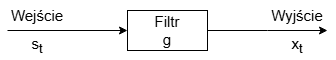
\includegraphics[width=0.5\textwidth]{pic/modele/model_sakad.png}
	\caption{Diagram modelu ruchów sakadowych z filtrem liniowym różniczkującym.}
	\label{fig:model-sakad}
\end{figure}

\subsubsection{Płynne podążanie}
\label{subsubsec:plynne-podazanie}

Płynne podążanie występuje gdy obserwator śledzi obiekt w ruchu, ruch ten oczywiście nie może być zbyt gwałtowny. Tego typu śledzenie jest przykładem systemu sterowania z ujemnym sprzężeniem zwrotnym. Do modelowania owych ruchów używana jest prosta pętla, którą można opisać nastepujacym równaniem \ref{eq:plynne-podazanie-pentla} w dziedzinie czasu.

\begin{align}
	h \cdot (s_t - x_t) &= x_{t+1} 
	\label{eq:plynne-podazanie-pentla}
\end{align}

Wejście $s_t$ to pozycja celu, wyjście $x_t$ to pożądana pozycja oka. Można zauważyć, że w tym przypadku nie jest wymagana transformacja informacji wejściowej na wyjściową, a jedynie zmodyfikowanie jej wartości, w związku z tym $h$ jest liniowym niezmiennym w czasie filtrem, czyli po prostu wzmocnieniem systemu. Przeprowadźmy teraz transformację Z na powyższym równaniu \ref{eq:plynne-podazanie-pentla} by uzyskać transmitancję systemu przedstawioną wzorem \ref{eq:plynne-podazanie-transmitancja}.

\begin{align} %!!!!!!!!!!!!!!!!!!!!!!!!!!!!TUTAJ JEST COŚ ŹLE Z TYM RÓWNANIEM%!!!!!!!!!!!!!!!!!!!!!!!!!!!!
	\mathcal{Z}\{h \cdot (s_t - x_t)\} &= \mathcal{Z}\{x_{t+1}\} \nonumber \\
	H(z) \cdot (S(z) - X(z)) &=  X(z) \nonumber \\ % POWINNO BYĆ CHYBA z \cdot X(z)
	H(z) \cdot S(z) - H(z) \cdot X(z) &=  X(z) \nonumber \\
	H(z) \cdot S(z) &= (H(z) + 1) \cdot X(z) \nonumber \\
	\frac{X(z)}{S(z)} &= \frac{H(z)}{H(z) + 1} \label{eq:plynne-podazanie-transmitancja}
\end{align}   %!!!!!!!!!!!!!!!!!!!!!!!!!!!!TUTAJ JEST COŚ ŹLE Z TYM RÓWNANIEM%!!!!!!!!!!!!!!!!!!!!!!!!!!!!

W ten sposób sygnał z receptorów oka służy za błąd, który następnie jest kompensowany w celu utrzymania obrazu w przestrzeni widzenia plamkowego. Diagram modelu przedstawiony jest na rysunku \ref{fig:model-smooth}.

\begin{figure}[htbp]
	\centering
	
\includegraphics[width=0.6\textwidth]{pic/modele/model_smooth.png}
	\caption{Diagram modelu płynnego podążania z liniowym sprzężeniem zwrotnym.}
	\label{fig:model-smooth}
\end{figure}

\subsubsection{Fiksacja}
\label{subsubsec:fiksacja}

Można zauważyć, że fiksacja jest procesem podobnym do płynnego podążania, z tą różnicą, że w tym przypadku obiekt jest nieruchomy. Jednakże proces ten nie da się bezpośrednio z sobą porównać i najprawdopodobniej nie ma wspólnego obwodu neuronalnego. Nasze komórki systemu wzrokowego są fizjologicznie wrażliwe na ruch, gdyby dany obiekt został unieruchomiony względem siatkówki, po krótkim czasie widzenie zaniknie. Powoduje to konieczność mikrosakad i innych mimowolnych, drobnych ruchów oczu. Można więc uznać, że model fiksacji jest podobny do modelu płynnego podążania, który próbuje utrzymać pozycję oka na danym punkcie, a mikrosakady i inne ruchy można uznać za szum w systemie kontrolnym, który można wyrazić jako $e_t = x_t - s_t$. Jest to losowa fluktuacja wokół punktu fiksacji, a jej wartość średnia pozostaje stała.

Ruch gałek ocznych i związane z nim widzenie jest bardzo szerokim tematem interdyscyplinarnym, na potrzeby tego projektu powyższe sformułowanie problemu, chociaż uproszczone i nie wyczerpujące, pozwala na zrozumienie w pełni istoty prezentowanego systemu.

% Osadzenie tematu w kontekście aktualnego stanu wiedzy

\section{Osadzenie tematu w kontekście aktualnego stanu wiedzy}
\label{sec:osadzenie-tematu-w-kontekscie-aktualnego-stanu-wiedzy}

Pomiar ruchu oczu był realizowany już w latach 70. XX wieku, nic dziwnego więc, że od tego momentu powstały różne techniki pozwalające na zebranie owych danych. Należy podkreślić, że metody te można podzielić na mierzące ruch oczu względem głowy, oraz takie które mierzą orientacje oczu w przestrzeni, czyli ,,punkt spojrzenia''. 

\subsection{Metody śledzenia ruchu oczu: przegląd historyczny i alternatywy}
\label{subsec:metody-sledzenia-ruchu-oczu-przeglad-historyczny-i-alternatywy}

Najstarszą z metod śledzenia ruchu oczu jest elektro-okulografia (EOG ang. \english{electrooculography}), wciąż wykorzystywana np. w badaniach klinicznych. Metoda ta polega na umieszczeniu elektrod na skórze twarzy wokół oczu i pomiarze różnicy potencjałów. Metoda ta z założenia mierzy ruch oczu względem głowy, ale można rozszerzyć ją o pomiar ruchu głowy dając możliwość wyliczenia punktu spojrzenia. 

Jedna z najdokładniejszych metod pomiaru ruchu oczu polega na umieszczeniu soczewki kontaktowej bezpośrednio na gałce ocznej. Soczewka ta powinna być odpowiednio duża, by objąć zarówno rogówkę jak i twardówkę, a na jej powierzchni umieszczany jest albo obiekt optyczny, którego zdaniem jest dokładne odbijanie światła lub dostarczenie wyraźnych kształtów potrzebnych do śledzenia, albo cewka wykonaną z drutu, która poruszając się w polu elektromagnetycznym pozwala na wykonanie pomiaru. Metoda ta jest bardzo dokładna, ale niezwykle inwazyjna i nieprzyjemna dla badanego, a także, podobnie do elektro-okulografii, mierzy ruch oczu względem głowy.

Wideo-okulografia i foto-okulografia tworzą razem szeroką grupę metod, które opierają się na analizie wyróżniających się cech oka podczas jego obrotu, takich jak: kształt źrenicy, pozycja granicy tęczówki i twardówki, czy odbicie światła (często podczerwonego) od rogówki. Metody te są nieinwazyjne, ale same w sobie nie pozwalają na określenie punktu spojrzenia, więc w celu wyznaczenia owego punktu często stosuje się unieruchomienie głowy osoby badanej, wyznaczenie punktu odniesienia np. przez odbicia światła od powierzchni oka, lub odpowiednią kalibrację np. prosząc osobę badaną o utrzymanie wzroku na danym punkcie ekranu.

\subsection{Analiza wideo z wykorzystaniem źrenicy i odbicia rogówkowego}
\label{subsec:analiza-wideo-z-wykorzystaniem-zrenicy-i-odbicia-rogowkowego}

Opisane metody wymagają unieruchomienia głowy (przez różnego rodzaju podpórki pod brodę lub głowę, albo nawet belki nagryzowe) lub zastosowanie dodatkowego sprzętu mierzącego ruch głowy, by wyznaczyć punkt spojrzenia. Jest to główna wada tych metod, jako że miejsce skupienia uwagi daje istotne informacje, które są najczęściej pożądane przez użytkowników okulografów. Dlatego metoda należąca do grupy wideo-okulografii, opierająca się na analizie obrazu wideo z kombinacją wykrycia źrenicy i odbicia rogówkowego, która pozwala na określenie punktu spojrzenia z dużą dokładnością, jest jedną z najpopularniejszych wyborów zarówno w świecie naukowym jak i komercyjnym. System prezentowany w tej pracy można zaliczyć do wideo-okulografii, z możliwością włączenia trybu z pomiarem odbicia rogówkowego, więc metoda ta zostanie omówiona szerzej od pozostałych.

Wykrywanie punktu spojrzenia metodą detekcji źrenicy i odbicia rogówkowego wymaga kilku kluczowych elementów. Potrzebna jest kamera wideo, która zarejestruje aktualny stan gałek ocznych oraz sprzęt, który pozwoli na przetworzenie obrazu i ostatecznie wykrycie interesujących cech, najlepiej w czasie rzeczywistym. Aktualnie oba wymienione elementy stają się coraz tańsze i bardziej wydajne, tak naprawdę większość osób posiada je w swoim smartfonie, co sprawia, że technika ta staje się bardziej dostępna dla szerokiego grona użytkowników. Aparatura ta jest także coraz bardziej miniaturyzowana, dzięki czemu aktualnie dostępne są systemy montowane na głowie, jak i montowane na biurku, które działają na tej samej zasadzie, różniąc się zasadniczo jedynie wielkością. Warto jednak zaznaczyć, że systemy montowane na głowie zazwyczaj posiadają także dodatkową kamerę wyznaczającą tak zwany POV (ang. point of view, czyli punkt widzenia), a spojrzenie jest monitorowane względem tego obrazu, w odróżnieniu do montowanych na biurku, które zazwyczaj mierzą spojrzenie względem pewnej powierzchni np. monitora. Należy omówić także źródło światła, którego odbicie rejestrowane jest podczas detekcji. Możliwe jest wykorzystanie punktowego źródła światła białego o odpowiednim natężeniu, jednakże może to prowadzić do dyskomfortu przy użytkowaniu lub nawet chwilowego oślepienia osoby badanej, wytrącając ją z stanu skupienia. W związku z tym najczęściej wykorzystywanym są źródła światła podczerwonego, które znajdują się w większości poza widzialnym spektrum, nie irytując oka, nie zakłócając procesu badania i pozwalając na użycie wyższego natężenia, operowanie na takim zakresie częstotliwości światła wymaga użycia specjalnych kamer, które są w stanie rejestrować światło IR (ang. infrared). 

Omawiane odbicie rogówkowe nazywane jest obrazem Purkinjego, budowa oka sprawia, że pojawiają się cztery odbicia, pierwsze to odbicie od zewnętrznej powierzchni rogówki (najbardziej widoczne), drugie od wewnętrznej powierzchni rogówki, trzecie od zewnętrznej powierzchni soczewki, a czwarte od wewnętrznej powierzchni soczewki. By poprawnie wyznaczyć punkt spojrzenia, wymagane jest wyznaczenie dwóch punktów odniesienia, pierwszy określający obrót oczu w oczodole, a drugi określający stałe położenie względem oczu. Pierwszym punktem zazwyczaj jest środek źrenicy, a drugim najczęściej jest pierwszy obraz Purkinjego, powstały przez źródło światła ustabilizowane względem głowy, lub powierzchni badanej. Przy nieruchomej głowie, ruch oczu odczytywany będzie jako zmieniająca się różnica pomiędzy tymi dwoma punktami, w odwrotnym przypadku, gdy głowa poruszy się, a oczy pozostaną w fiksacji na danym punkcie, dla systemu montowanego na biurku różnica ta pozostanie stała, a dla systemu montowanego na głowie, różnica będzie zmieniać się proporcjonalnie do zmiany punktu widzenia. Istnieją także okulografy piątej generacji z technologią DPI (ang. Dual Purkinje Image), mierzą one dodatkowo czwarty obraz Purkinjego, dzięki temu, mogą rozróżniać ruchy translacyjne oka od ruchów rotacyjnych, jako że przy translacji obrazy Purkinjego poruszają się o tą samą odległość, a przy rotacji zmieniają swoje rozdzielenie, co zwiększa precyzję pomiaru, ale wymaga bardziej skomplikowanego oprogramowania, a także unieruchomienie głowy może okazać się konieczne.

\section{Studia literaturowe}
\label{sec:studia-literaturowe}

% UWAGA - Czy cytat nie powinien być przeniesiony na koniec akapitu?
Powyższe sformułowanie problemu i jego osadzenie w kontekście aktualnego stanu wiedzy zostało przedstawione w oparciu o książkę ,,Eye Tracking Methodology: Theory and Practice'' autorstwa Andrew T. Duchowskiego \cite{bib:eye-tracking-methodology}. Książka ta dogłębnie omawia temat śledzenia ruchu oczu, pozwalając na zgłębienie zarówno podstaw procesów wzrokowych w kontekstach różnych dziedzin naukowych, a także szeroko omawia praktykę pomiaru ruchu oczu. Powyższa analiza tematu skupia się jedynie na najistotniejszych aspektach, które pozwolą na zrozumienie istoty prezentowanego systemu, a wiedzę na ich temat można poszerzyć lekturą wspomnianej książki.

Eye-tracking staje się coraz bardziej dostępny, co sprawia że technologia ta znajduje zastosowanie w wielu obszarach, zarówno w badaniach naukowych jak i do użytku konsumenckiego czy komercyjnego. Część producentów owych systemów udostępnia publikacje naukowe, w których zostały one wykorzystane, a ich analiza przedstawia różne rozwiązania omawianego tematu.

\subsection{Metoda źrenicy i odbicia rogówkowego w badaniach}
\label{subsec:metoda-zrenicy-i-odbicia-rogowkowego-w-badaniach}

Jednym z przedstawicieli firm skupiających się na analizie zachowań ludzkich jest iMotions, wyróżniając się modularnym systemem z centralnym hubem. Firma ta oferuje biosensory w formie modułów, pozwalające na np. śledzenie oczu, analizę wyrazu twarzy, rejestrowanie aktywności elektrycznej mózgu i rejestrowanie aktywności serca. Dane zebrane przez różne czujniki są integrowane w jednym oprogramowaniu co pozwala badaczom na prostą synchronizację i analizę danych w jednym systemie \cite{bib:iMotions-about-us}. Jednak mimo tak obszernego asortymentu biosensorów, to właśnie moduł śledzenia wzroku na ekranie (montowany na biurku) był wykorzystywany najczęściej w badaniach naukowych, z czego eye-tracking był najczęściej wykorzystywany w systemach jednomodułowych \cite{bib:iMotions-2023-report}. Pokazuje to jak uniwersalnym i podstawowym narzędziem jest eye-tracker w badaniach behawioralnych i nie tylko. 

Jednym z przeprowadzonych badań z użyciem technologii iMotions było ,,Using Psychophysiological Data to Facilitate Reflective Conversations with Children about their Player Experiences''. Podobne badania były przeprowadzane wielokrotnie w stosunku do osób dorosłych, jednak w przypadku grupy badanej składającej się z dzieci, badacze mogą napotkać znaczny problem z odpowiednim zrozumieniem wywiadu, w którym uczestnicy dzielą się swoimi wrażeniami z przeprowadzonej rozgrywki. Omawiane badanie miało głównie na celu sprawdzenie czy zebrane dane z biosensorów są wstanie wspomóc refleksje dzieci na temat ich doświadczenia w grze i czy dzieci napotkają problemy z interpretacją prezentowanych danych, jako że odnoszenie się do stanu psychofizjologicznego może zminimalizować problem z komunikacją pomiędzy dzieckiem, które posiada ograniczone umiejętności werbalne, a badaczem. 

Do śledzenia ruchu gałek ocznych na ekranie zastosowano okulograf Smart Eye AI-X o częstotliwości próbkowania $60 \ \unit{\hertz}$, posługujący się techniką detekcji źrenic i odbicia rogówkowego, pozwalając na sporą swobodę ruchu głowy w przestrzeni $35 \, \unit{\centi\metre}$ na $30 \, \unit{\centi\metre}$, jednocześnie posiadając dokładność (różnica pomiędzy rzeczywistą pozycją spojrzenia a pozycją spojrzenia zarejestrowaną przez okulograf) $\ang{0.5}$ i precyzję (średnia kwadratowa punktów mierzonych w jednej pozycji oka) $\ang{0.1}$, zwracając dane wyjściowe binokularowe z wskaźnikiem jakości zawierające: punkt spojrzenia, średnicę źrenicy oraz znacznik czasowy \cite{bib:iMotions-smart-eye-ai-x}. Oprócz tego zastosowano moduł rejestrujący aktywność sercową, analizujący wyrazy twarzy oraz mierzący reakcję skórno-galwaniczną. 

Badanie składało się z dwóch etapów, wpierw zebrano dane w laboratorium podczas gdy badane dzieci grały w dwie gry oraz podczas wywiadów bezpośrednio po zakończonej rozgrywce, a następnie prezentowano badanym momenty z pierwszego etapu z uwzględnieniem danych z biosensorów i zadawano pytania o ich doświadczenia. Badania wskazały, że dzieci są wstanie zrozumieć i odpowiednio odnieść się do prezentowanych danych psychofizjologicznych, a oparcie się o nie może pomóc w zwerbalizowaniu swojego doświadczenia i informacji zwrotnej przez badane dzieci. Dzieci nie miały problemu z zrozumieniem większości pomiarów za wyjątkiem reakcji skórno-galwanicznej, jednakże dane eye-trackingowe były swego rodzaju wyjątkiem, jako że nie prezentowały bezpośrednio doświadczenia i uczuć związanych z danym wydarzeniem w grze, a raczej dawały wgląd w strategię objęta przez dziecko zmagające się z aktualnym wyzwaniem, mimo tego prezentowane śledzenie punktu spojrzenia było naturalne w interpretacji przez badanych \cite{bib:iMotions-children}. Publikacja ta pokazuje jak okulografia może zostać skutecznie użyta w badaniach naukowych, ale przede wszystkim przedstawia istotność tej techniki w zastosowaniach komercyjnych np. testując doświadczenia graczy przy produkcji gier wideo dla różnych grup wiekowych.

\subsection{Porównanie z video-okulografią z użyciem kamerki internetowej}
\label{subsec:porownanie-z-video-okulografia-z-uzyciem-kamerki-internetowej}

Warto omówić także przykłady systemów opierających się jedynie na analizie wideo z kamerki internetowej, jako że system prezentowany w tej pracy działa przede wszystkim na tej zasadzie. Ten typ okulografii opartej na analizie wideo w czasie rzeczywistym cieszy się dużą popularnością wśród konsumentów, jako że sprzętowo wymaga od użytkownika posiadanie jedynie komputera z wbudowaną lub zewnętrzną kamerą, a całość przetwarzania obrazu, wyświetlania i zbierania danych oraz wyliczania punktu spojrzenia realizowane jest przez software producenta eye-trackera. Istotność takiego rozwiązania pojawia się także gdy przeprowadza się badania na dużej grupie, jako że osoba badana sama dostarcza sprzęt w formie laptopa czy nawet smartfona, a zbierane dane przesyłane są do badaczy przez internet, eliminując potrzebe stwarzania przestrzeni laboratoryjnej i planowania dogodnych terminów eksperymentów. Dlatego firmy specjalizujące się w okulografii, często oferują także oprogramowanie do śledzenia ruchu gałek ocznych przez kamerkę internetową, jak wspomniana już wcześniej firma iMotions. Często także dostępne są rozwiązania od niezależnych dostawców oprogramowania, które za subskrypcją, opłatę, lub całkowicie bezpłatnie oferują śledzenie punktu spojrzenia przez kamerę komputera, jednym z takich programów, który zostanie omówiony jest darmowy GazeRecorder. 

W publikacji ,,WebET 3.0 -Validation Study Report'' przeprowadzono badania sprawdzające efektywność śledzenia ruchu gałek ocznych przez oprogramowanie WebET 3.0 firmy iMotions z wykorzystaniem kamerek internetowych uczestników, bez względu na ich oświetlenie, rozdzielczość kamery czy prędkość internetu. Grupa badana została utworzona tak by reprezentować różne pochodzenie, wiek, płeć i kolor oczu, uczestnicy mogli także posiadać owłosienie twarzy oraz nosić okulary. By stworzyć punkty odniesienia pokazano badanym gify z kotami oraz emotikony w tych samych miejscach, a następnie obliczono dokładność mierząc odległości pomiędzy zarejestrowanymi punktami spojrzenia, a ustalonymi punktami odniesienia. 

Wyniki dokładności wskazały, że system iMotions jest niezależny na zmienne wynikające z pochodzenia, koloru oczu, wieku, płci oraz owłosienia twarzy, jednak posiadanie okularów mogło wpływać na wynik śledzenia, rodzaj i natężenie oświetlenia także nie wpływał znacząco na działanie WebET 3.0. Ponad $90\%$ uczestników posiadało dokładność mniejszą od $\ang{5}$ dokładności, $70\%$ badanych posiadało dokładność mniejszą od $\ang{3}$ dokładności, a mediana dokładności wynosiła $\ang{2.08}$ \cite{bib:iMotions-WebET}. Dokładność alternatywnego darmowego oprogramowania GazeRecorder została zaprezentowana w przeglądzie systematycznym i wynosiła $\ang{1,43}$ z możliwością poprawy do $\ang{1,3}$ przez unieruchomienie głowy, pozwalając na noszenie okularów za wyjątkiem okularów antyrefleksyjnych \cite{bib:GazeRecorder-Review}. 

\subsection{Podsumowanie metod w literaturze}
\label{subsec:Podsumowanie-metod-w-literaturze}

Metoda śledzenia ruchu gałek ocznych przy użyciu źrenicy i odbicia rogówkowego w podczerwieni znacznie przewyższa -- pod względem dokładności -- metodę polegającą na kamerce internetowej, w związku z tym przy badaniach skupiających się na analizie gęsto ułożonych informacji wyspecjalizowany okulograf może być bardziej pożądany. Jednakże aktualna dostępność sprzętu i oprogramowania potrzebnego do śledzenia z użyciem kamerki internetowej daje możliwość na bardziej obszerne zastosowania, a ich dokładność pozwala na efektywne śledzenie punktu spojrzenia w przypadkach gdy informacje są ułożone z odpowiednimi dystansami.





\begin{itemize}
\item sformułowanie problemu
\item osadzenie tematu w kontekście aktualnego stanu wiedzy (\english{state of the art}) o poruszanym problemie
\item  studia literaturowe \cite{bib:artykul,bib:ksiazka,bib:konferencja,bib:internet} -  opis znanych rozwiązań (także opisanych naukowo, jeżeli problem jest poruszany w publikacjach naukowych), algorytmów, 
\end{itemize}


%%%%%%%%%%%%%%%%%%%%%%%%





%--------------------------------------
%
%
% TODO: krótkie wprowadzenie na początku każdej sekcji/rozdziału
%
% Status: 99%
%--------------------------------------
\chapter{Wymagania i narzędzia}
\label{ch:wymagania-i-narzedzia}

\section{Wymagania funkcjonalne}
\label{sec:wymagania-funkcjonalne}

Postawienie konkretnych granic funkcjonalnych projektu jest kluczowym elementem tworzenia rozwiązania. Działają one na zasadzie zabezpieczenia przed usprawnianiem i rozszerzaniem projektu bez końca, a także pozwalają na skupienie uwagi inżyniera na istotnych aspektach. Można zauważyć korelację pomiędzy rolą wymagań funkcjonalnych w tworzeniu projektu, a plamką żółtą w oku omawianej w podrozdziale \ref{sec:sformulowanie-problemu}, oba elementy dbają o to by wiele informacji zostało przefiltrowane do tych, które są najważniejsze.

\subsection{Limitacje sprzętowe i środowiskowe}
\label{subsec:Limitacje-sprzetowe-i-srodowiskowe}

Do śledzenia ruchu gałek ocznych używany jest bardzo szeroki wachlarz sprzętów i związanych z nimi rozwiązań technicznych omówionych w podrozdziałach \ref{sec:osadzenie-tematu-w-kontekscie-aktualnego-stanu-wiedzy} i \ref{sec:studia-literaturowe}, jednakże w założeniu tego projektu było opierać się na systemie wizyjnym, co pozwala na ograniczenie znanych metod do video-okulografii. Kolejną ustaloną limitacją było opieranie się jedynie na aktualnie dostępnym sprzęcie, którym był laptop ASUS Vivobook 15 z wbudowaną kamerką internetową USB2.0 HD UVC o częstotliwości próbkowania $30 \ \unit{\hertz}$, podczas korzystania z kamery automatycznie włączane było także niewielkie źródło światła przylegające z jej prawej prawej strony. Tego typu laptop z wbudowaną kamerą reprezentuje jakość sprzętu często używaną do zastosowań biurowych i użytku własnego, dlatego też założono, że źródła światła powinny zostać ograniczone do podstawowego oświetlenia wewnętrznego, tworząc środowisko typowe do pokoju mieszkalnego, w którym korzysta się z komputera.

\subsection{Wykorzystanie platform i narzędzi programistycznych}
\label{subsec:Wykorzystanie-platform-i-narzedzi-programistycznych}

By uprościć użycie komputera (wspomnianego w punkcie \ref{subsec:Limitacje-sprzetowe-i-srodowiskowe}), zdecydowano się na pozostaniu przy już zainstalowanym systemie operacyjnym, którym jest Windows 11. Podobnie postawiono wymaganie względem edytora kodu źródłowego i systemu kontroli wersji, jako że użycie znajomego środowiska, które już jest zainstalowane i było wcześniej używane na wykorzystanym laptopie, pozwala na szybkie zamknięcie przygotowań do pracy. W związku z tym skupiono się na rozwiązaniach, które są kompatybilne z edytorem tekstu Visual Studio Code i klientem Git z graficznym interfejsem użytkownika GitHub Desktop, jako że narzędzia te ściśle z współpracują z sobą i serwisem hostingowym GitHub tworząc intuicyjną i znajomą w użyciu całość. Stawianym wymaganiem do języka programowania, oprócz wspomnianej kompatybilności, jest jego popularność, uniwersalność, klarowność i szeroki wybór bibliotek. Język o takich cechach znacznie zwiększy produktywność, uprości stosowanie bardziej skomplikowanych narzędzi i pozwoli na efektywne uczenie się i rozwiązywanie problemów opierając się na społeczności użytkowników. Zalety te wspomogą uzyskanie natychmiastowych rezultatów pracy oraz skoncentrowanie uwagi na poprawie i rozwój funkcjonalności systemu. Łatwo dostępnym i popularnym językiem o wysokim poziomie abstrakcji jest Python, który jest oficjalnie wspierany przez Visual Studio Code. Język ten posiada możliwość korzystania z biblioteki OpenCV, która daje dostęp do wielu rozwiązań przetwarzających obraz. Ostatnim, bardziej personalnym atutem proponowanego języka, jest niewielkie ówczesne doświadczenie programowania w nim, a co za tym idzie szansa na zyskanie cennych umiejętności w trakcie pracy.

\subsection{Zakres działania systemu}
\label{subsec:zakres-dzialania-systemu}

Nakreślone limitacje w punkcie \ref{subsec:Limitacje-sprzetowe-i-srodowiskowe} i \ref{subsec:Wykorzystanie-platform-i-narzedzi-programistycznych} odpowiednio ograniczyły możliwe rozwiązania, pozwalając na ustalenie realnych funkcjonalności programu. Aspektem, który przede wszystkim determinuje stopień skomplikowania stawianych wymagań, jest ograniczony czas na wykonanie omawianego systemu. W związku z tym, rozwiązaniem, które może zapewnić użyteczność planowanego systemu, nawet w przypadku jego niepełnego ukończenia, jest skoncentrowanie się na podstawowych funkcjonalnościach. Dzięki temu powstanie solidny szkielet projektu, oferujący funkcje dostępne na danym etapie prac. W konsekwencji zakres działania systemu śledzącego ruch oczu przedstawia się następująco:

\begin{enumerate}
	\item Przetwarzanie obrazu z kamery powinno odbywać się w czasie rzeczywistym. Dzięki takiemu rozwiązaniu nie będzie potrzebne nagrywanie, a także pozwoli to na weryfikację pracy systemu w trakcie użytkowania. Biblioteka OpenCV posiada wiele rozwiązań, które pozwalają na operowaniu na obrazie w czasie rzeczywistym.
	\item Proces śledzenia ruchu gałek ocznych powinien przebiegać poprzez wpierw wykrycie twarzy, następnie w rejonie twarzy przeprowadzanie detekcja oczu, a dopiero w rejonie oczu dojdzie do wykrycia źrenicy. Dzięki takiemu założeniu obraz będzie stopniowo ograniczany do rejonu zainteresowania, gwarantując ograniczenie błędnych detekcji.
	\item System powinien działać w sposób binokularny, pozwalając na wykrycie i zidentyfikowanie obu oczu (a następnie źrenic) z rozróżnieniem lewego i prawego oczodołu. Dzięki takiemu rozwiązaniu dane wyliczane przez system będą skategoryzowane, zabezpieczając przed błędami i niespójnościami w analizie.
	\item Wykrywanie źrenic powinno być uniwersalne względem oświetlenia otoczenia. Oczywistym jest, że skrajnie złe oświetlenie uniemożliwi poprawne działanie, ale program powinien cechować się pewnym stopniem elastyczności, nie wymuszając użytkowania w jednym konkretnym środowisku.
	\item By obliczyć przemieszczenie źrenicy musi zostać wyznaczony umowny punkt odniesienia względem powierzchni, na której skupiona jest uwaga, punkt ten powinien być odporny na niewielkie ruchy głowy. Dodatkowym atutem będzie możliwość prostej kalibracji owego punktu. Jest to kluczowy element pozwalający na detekcję ruchu oczu.
	\item Wyznaczanie ruchu oczu poprzez jedynie umowny punkt odniesienia, o ograniczonej możliwości weryfikacji poprawności pomiaru, nie jest rozwiązaniem idealnym i może być niewystarczające dla bardziej zaawansowanych użytkowników. W związku z tym system powinien oferować opcję wyznaczenia ruchu gałek ocznych względem realnego punktu odniesienia np. poprzez zastosowanie dodatkowego sprzętu.
	\item Wyliczone przemieszczenie źrenicy w czasie rzeczywistym powinno zostać zapisane do pliku, który pozwoli na analizę zebranych danych w tym pozycję źrenicy, indeks wskazujący przynależność do odpowiedniego oka oraz moment czasowy zebranego pomiaru.
\end{enumerate}


\section{Wymagania niefunkcjonalne}
\label{sec:wymagania-niefunkcjonalne}

Jak ustalono w punkcie \ref{subsec:zakres-dzialania-systemu} projekt ten ma skupić się na utworzeniu solidnego szkieletu programu, takie rozwiązanie kładzie nacisk przede wszystkim na funkcjonalność i wymusza jednocześnie zastosowanie jedynie najważniejszych elementów interfejsu, pozwalając użytkownikowi na wykorzystanie jego pełni możliwości. Wymagania niefunkcjonalne mogą w takim razie być skromniejsze względem funkcjonalnych, ale wciąż należy je dokładnie określić by uniknąć utraty kluczowych elementów przez zaniedbanie tej części. Wymagania te prezentują się następująco:

\begin{enumerate}
	\item Program powinien wyświetlać obraz z kamery, jest to najbardziej podstawowe wymaganie, ale także najbardziej istotne. Obserwacja obrazu daje informację zwrotną użytkownikowi, pozwalając na szybką weryfikację działania kamery, a także analizę przystępności otoczenia, w którym dokonuje śledzenia.
	\item Jako że możliwe jest uszkodzenia pliku programu, lub braku odpowiedniego sprzętu wymaganego do przeprowadzenia detekcji, istotnym jest wdrożenie podstawowej kontroli błędów zwracającej odpowiednią informacje i zakańczając działanie programu w przypadku wykrycia nieprawidłowości. Informacja ta powinna nakierować użytkownika na źródło problemu, pozwalając na łatwiejsze dojście do jego rozwiązania.
	\item W punkcie \ref{subsec:zakres-dzialania-systemu} wymieniono różne funkcjonalności programu, część z nich (np. rodzaj wyznaczania punktu odniesienia) z reguły nie będzie działać równolegle, wymaga to więc prostego sposobu na kontrolowanie, która z użyteczności będzie w tym momencie wykorzystywana. 
	\item Podczas działania systemu śledzenia ruchu gałek ocznych dokonywana będzie detekcja kilku elementów, takich jak twarz, oczy oraz źrenice, istotnym aspektem wizualnym jest podkreślenie tych obszarów, dając możliwość na naturalną kontrolę działania rozwiązania na każdym jego etapie. Dodatkowo warto zaznaczyć punkt odniesienia i punkt środka źrenicy, obrazując dzielący ich dystans. Jest to duża ilość informacji, która może zaciemnić obraz z kamery, program powinien w związku z tym zadbać o maksymalną przejrzystość.
	\item Poza bardziej zrozumiałym empirycznie obrazowaniem działania systemu śledzącego, takim jak zaznaczanie obszarów detekcji, przydatnym może okazać się wizualizowanie technicznego aspektu wykrywania, prezentując to jak komputer odbiera i przekształca obraz z kamery. Tak przedstawione wyniki, chociaż mniej czytelne dla osób niezaznajomionych, pozwolą użytkownikowi na poprawę działania programu pod jego własne preferencje.
	\item Przeglądanie zebranych danych może być dużym wyzwaniem, jako że komercyjnie dostępne kamery internetowe mogą rejestrować obraz $30$ lub nawet $60$ razy na sekundę, co przy dłuższym śledzeniu generuje obszerną ilość pomiarów. Z tego powodu wymagana jest wizualizacja zebranych danych w prosty sposób np. przez wykresy czasowe. Takie rozwiązanie pomoże w dalszej analizie i potencjalnej obróbce pomiarów.
\end{enumerate}

\section{Przypadki użycia}
\label{sec:przypadki-uzycia}

Wymagania funkcjonalne i niefunkcjonalne omawiane w podrozdziale \ref{sec:wymagania-funkcjonalne} i \ref{sec:wymagania-niefunkcjonalne} pozwalają dokładnie opisać konkretne elementy systemu, ale mogą utrudniać zrozumienie całości. Diagram UML (Unified Modeling Language) przypadku użycia pozwala na łatwe zobrazowanie każdego elementu w kontekście całości programu, dopełniając analizę stawianych wymagań. Diagram przypadku użycia prezentowanego systemu widoczny jest na rysunku \ref{fig:UML-use-case}. 

\begin{figure}[htbp]
	\centering
	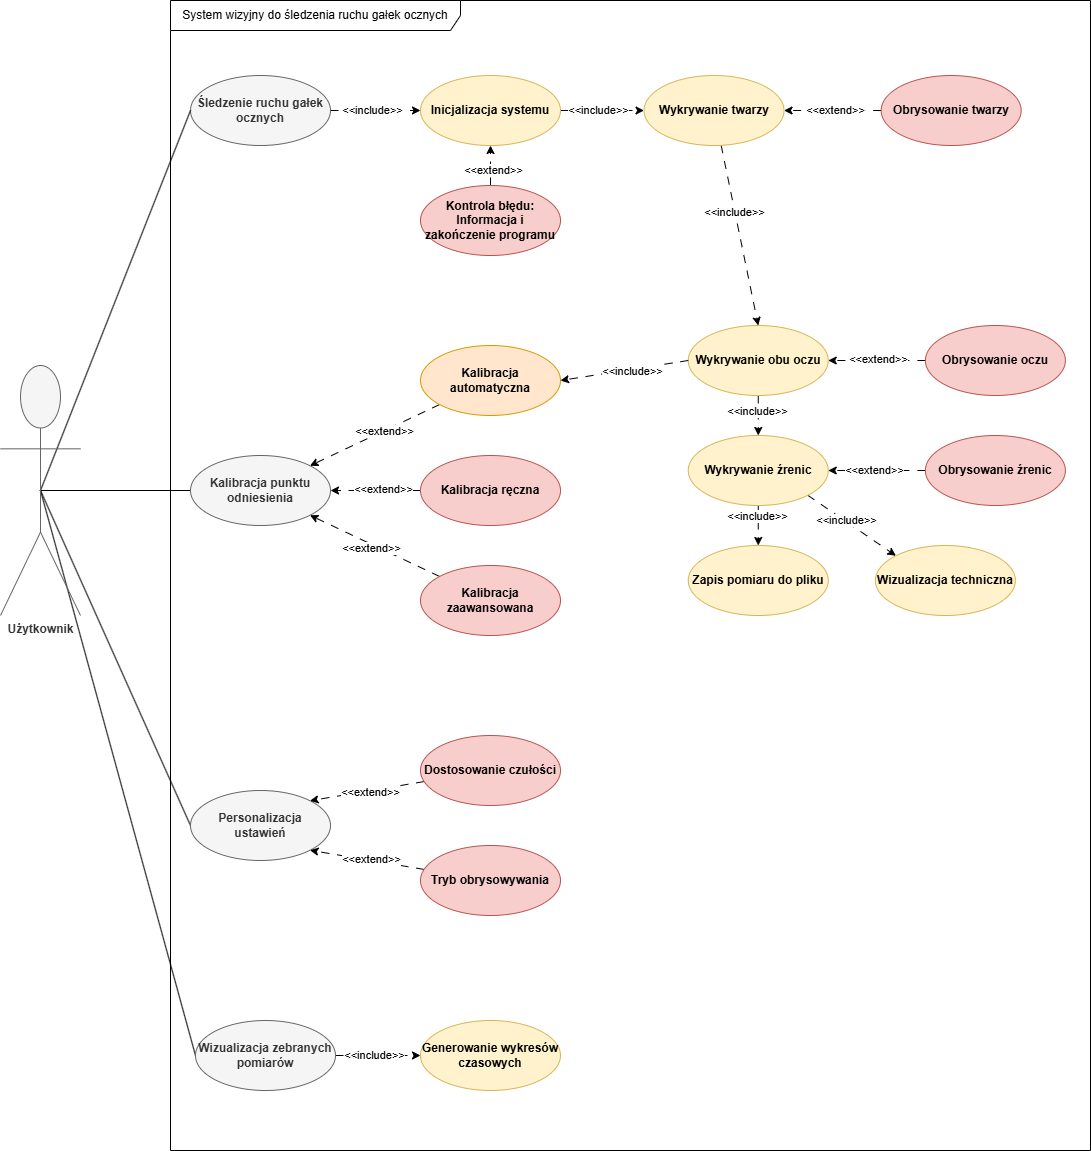
\includegraphics[width=\textwidth]{pic/use case/use case diagram.png}
	\caption{Diagram UML przypadku użycia systemu do śledzenia ruchu gałek ocznych.}
	\label{fig:UML-use-case}
\end{figure}

Diagram na rysunku \ref{fig:UML-use-case} prezentuje po lewej użytkownika, który pełni rolę aktora wchodzącego w interakcję z systemem wizyjnym do śledzenia ruchu gałek ocznych. Użytkownik może oddziaływać na system na cztery sposoby, rozpoczynając śledzenie, kalibrując punkt odniesienia, personalizując ustawienia oraz wizualizując zebrane pomiary, akcje są ustawione od góy w kolejności sugerującej korzystanie z programu. Śledzenie ruchu gałek ocznych rozpoczyna się inicjalizacją systemu, jeśli program nie napotka błędu, rozpoczyna wykrywanie obszarów twarzy. Zawężanie obszarów zainteresowań następuje sekwencyjnie, dopiero gdy pojawi się twarz można będzie szukać oczu i następnie źrenic. Gdy oczy zostaną wykryte, automatycznie utworzony zostanie punkt odniesienia, a gdy detekcja przebiegnie w całości pomyślnie, zapisany zostanie pomiar pozycji źrenicy względem punktu odniesienia oraz zostanie wyświetlony przetworzony obraz pomagający w dostosowaniu czułości. Użytkownik może następnie przeprowadzić kalibrację punktu odniesienia ręcznie lub kalibracją zaawansowaną, może też w każdej chwili wrócić do kalibracji automatycznej. Personalizacja, pozwalająca dostosować czułość detekcji oraz opcje obrysowania wykrytych rejonów twarzy, może okazać się konieczna w przypadku różnych warunków oświetleniowych, lub zmieniających się preferencji użytkownika. Po udanej sesji śledzenia ruchu gałek ocznych, użytkownik może zdecydować się na wizualizację zebranych pomiarów, generując wykresy czasowe. W ten sposób omawiany diagram UML przedstawia symbolicznie pełen zakres interakcji użytkownika z systemem oraz kolejność operacji, obrazując działanie aplikacji w typowym scenariuszu.

\section{Narzędzia i metody wykorzystane w pracy}
\label{sec:Narzedzia-i-metody-wykorzystane-w-pracy}

\subsection{ASUS Vivobook 15}
\label{subsec:ASUS-Vivobook-15}

Projekt prezentowany w tej pracy skupia się przede wszystkim na oprogramowaniu, dlatego sprzęt wykorzystany do jego zrealizowania zamyka się na laptopie z wbudowaną kamerką internetową, który jest także źródłem stawianych wymagań w punkcie \ref{subsec:Limitacje-sprzetowe-i-srodowiskowe}. Jest to ASUS Vivobook 15 D1502YA-BQ309 posiadający ośmiordzeniowy procesor AMD Ryzen 7 7730U z zintegrowanym układem graficznym ATI AMD Radeon Graphics. Notebook ten oryginalnie stosowany był do nauki i programowania, co pozwoliło na szybkie przystosowanie go do pracy nad prezentowanym rozwiązaniem, wpasowuje się on również w założenie limitacji sprzętowych użytkowników. Wbudowana kamera to USB2.0 HD UVC WebCam producenta Realtek, urządzenie te rejestruje obraz w $30$ klatkach na sekundę w rozdzielczości $1280 \times 720$, posiada także diodę światła białego, która ułatwia śledzenie w niesprzyjających warunkach oświetleniowych i tworzy widoczne na obrazie odbicie rogówkowe. Mimo że nie jest to kamera specjalistyczna, jej parametry są wystarczające do realizacji założeń projektu, a podobne specyfikacje są powszechne w kamerach wbudowanych w laptopy, co sprawia, że opracowane rozwiązanie może być łatwo wdrożone przez użytkowników bez konieczności zakupu dodatkowego sprzętu.

\subsection{Narzędzia programistyczne}
\label{subsec:Narzedzia-programistyczne}

\subsubsection{Github Desktop i Github}

Projekt o takiej skali wymaga użycia systemu kontroli wersji, by zabezpieczyć przed utratą postępów i pozwalając na bezproblemowe testowanie nowych funkcji. Do przechowywania kodu w chmurze i zabezpieczenia go na zdalnych serwerach wykorzystano hosting GitHub. W celu ułatwienia pracy z systemem kontroli wersji Git użyto aplikacji GitHub Desktop, zapewniającej graficzny interfejs użytkownika, co pozwoliło na wygodniejsze korzystanie z poleceń Git, zatwierdzanie zmian z odpowiednimi wiadomościami, operowanie na gałęziach repozytorium, analizowanie historii zmian oraz synchronizację lokalnego repozytorium z jego zdalnym odpowiednikiem na GitHubie.

\subsubsection{Visual Studio Code (VS Code)}

Visual Studio Code to edytor kodu źródłowego, który świetnie integruje się z Github desktop i przez to także z Github. VS Code mimo niskich wymagań systemowych, oferuje wiele funkcjonalności, co pozwoliło na wykorzystanie go jako główne narzędzie programistyczne. Dzięki kolorowaniu składni, automatycznym podpowiedzą i uzupełnianie kodu, edytor ten przyśpiesza pracę i ogranicza ilość błędów. Obszerna biblioteka wtyczek, pozwala na dostosowanie VS Code do własnych potrzeb, np. dodając obsługę języków programowania takich jak Python, czy \LaTeX. Wbudowana integracja z systemem kontroli wersji podkreśla zmodyfikowane pliki, ułatwiając zarządzanie repozytorium. Wbudowana obsługa terminala oraz zaawansowane debugowanie z kontrolą punktu wstrzymania, inspekcją zmiennych i śledzeniem wykonywania kodu w czasie rzeczywistym pozwala na szybką kompilację i naprawę programu, zwłaszcza napisanego w języku Python \cite{bib:VSCode-Essentials}. Podsumowując, Visual Studio Code okazał się niezastąpionym narzędziem w procesie tworzenia zarówno projektu, jak i niniejszej pracy, pozwalając nie tylko na ułatwioną organizację, ale również zwiększoną efektywność.

\subsubsection{Python 3.13.0}

Python to wysokopoziomowy język programowania, który charakteryzuje się czytelną i intuicyjną składnią. Cechuje go dynamiczne typowanie, przypisując typy zmiennych w trakcie działania programu oraz automatyczne zarządzanie pamięcią. Największym atutem Pythona jest jego popularność i łatwość nauki, co sprawia, że wokół tego języka powstała spora społeczność programistów. Dzięki temu w sieci można znaleźć liczne fora dyskusyjne, obszerne dokumentacje, a także poradniki i kursy wideo, które okazały się niezastąpionym wsparciem w realizacji niniejszej pracy. Python posiada również obszerną bibliotekę standardową oraz szeroki wybór wysokiej jakości bibliotek zewnętrznych, które oferują gotowe rozwiązania dla niemal każdego zagadnienia programistycznego. Dzięki nim możliwe jest realizowanie złożonych zadań, takich jak analizy danych i przetwarzania obrazów, często przy użyciu zaledwie kilku linijek kodu \cite{bib:Python-a-byte}. W efekcie, Python zaopatrzony w odpowiednie biblioteki, w przypadku realizacji omawianego rozwiązania, okazał się jedynym językiem programowania potrzebnym do implementacji wszystkich funkcjonalności systemu.

\subsubsection{OpenCV}

OpenCV jest otwartą biblioteką, która posiada ponad $2500$ zoptymalizowanych algorytmów, w tym rozpoznawania obrazu i uczenia maszynowego. Jej dodatkowym atutem jest dokładna dokumentacja i szeroka baza użytkowników aktywnie dzielących się swoimi obserwacjami i wyjaśnieniami na forach dyskusyjnych, pozwalając na sprawne wykorzystanie ogromnego potencjału tej biblioteki  \cite{bib:OpenCV-about}. To właśnie dzięki niej możliwe było większość operacji związanych z obrazem w czasie rzeczywistym, od przechwycenia go przez kamerę, przez wykrycie oraz obrysowanie twarzy i oczu, po binaryzację i operacje morfologiczne.

\subsubsection{NumPy}

NumPy to otwarta biblioteka zapewniająca obsługę dużych wielowymiarowych i jednolitych macierzy oraz tablic. OpenCV wykorzystuje i przekazuje tablice NumPy w swoich funkcjach, pozwalając na integrację obu bibliotek i łatwe operowanie na obrazach w formie macierzy \cite{bib:NumPy-quick-start}. Popularność tej biblioteki, zwłaszcza w użyciu wraz z OpenCV, sprawia, że jest szeroko omawiana przez społeczność programistyczną, co przekłada się na dużą liczbę poradników i zasobów edukacyjnych \cite{bib:NumPy-OpenCV}. Co za tym idzie jej zastosowanie w projekcie gwarantowało dostępność wsparcia w rozwiązywaniu potencjalnych problemów.

\subsubsection{Matplotlib}

Matplotlib jest biblioteką do tworzenia wykresów w języka Python, bezproblemowo współpracująca z NumPy. Użycie jej razem z modułem Pyplot pozwala na wizualizacje wyników z interfejsem podobnym do programu MATLAB \cite{bib:Matplotlib-pyplot}. Zastosowanie jej w pracy jest podparte dopełnieniem wcześniej wymienionych bibliotek, a także zbieżnością z znanym już środowiskiem MATLAB.

\subsubsection{pandas}

Pandas to biblioteka do analizy i manipulacji danymi, posiadająca narzędzia do czytania i zapisywania danych w plikach CSV oraz plikach tekstowych \cite{bib:Pandas-about}. Podczas śledzenia ruchu gałek ocznych generowana i zapisywana jest duża ilość danych, a biblioteka ta pozwala na łatwe wydobycie ich z pliku i wykorzystanie w dalszej części programu.

\subsubsection{Time}

Time jest częścią podstawowej biblioteki Python i nie wymaga dodatkowej instalacji przed użyciem, służy do wykonywanie operacji związanych z czasem. Zbierany pomiary muszą być zapisywane razem z momentem czasowym, by pozwolić na pełną analizę, jest to nieskomplikowane zadanie, które można rozwiązać z użyciem tej biblioteki opierając się na oficjalnej dokumentacji Python \cite{bib:time-Python}.

\subsubsection{PyInstaller 6.11.1}

Następnym krokiem, który warto wykonać po zakończeniu prac nad rozwiązaniem, jest ułatwienie jego dystrybucji i użytkowania. W tym celu wykorzystano PyInstaller, który umożliwia spakowanie skryptu Pythona i wszystkich jego zależności do samodzielnego pliku wykonywalnego (exe). Dzięki temu użytkownicy mogą uruchomić program bez konieczności instalowania interpretera Pythona ani dodatkowych modułów. Warto jednak zaznaczyć, że użyto PyInstaller w wersji na system operacyjny Windows, a oprogramowanie te nie pozwala na kompilację krzyżową (czyli wymaga tego samego systemu od użytkownika) \cite{bib:PyInstaller-manual}. Taka forma dystrybucji znacząco ułatwia udostępnianie aplikacji, a także eliminuje problemy związane z niedopatrzeniem w konfigurowaniu środowiska.

\subsection{Metodyka pracy nad projektem}
\label{subsec:Metodyka-pracy-nad-projektem}

Praca nad projektem przebiegała w sposób iteracyjny, co przypomina metodykę zwinnego wytwarzania oprogramowania, a w szczególności podejście stosowane w Scrum, które opiera się na empiryzmie. Proces ten polegał na wyznaczaniu pojedynczych zadań do realizacji, implementowaniu ich rozwiązań, a następnie analizowaniu wyników i dostosowywaniu kolejnych kroków \cite{bib:Scrum-guide}. Oznacza to, że stawiane wymagania i używane narzędzia, omawiane w rozdziale \ref{ch:wymagania-i-narzedzia}, także były poszerzane w sposób iteracyjny w czasie realizacji projektu. Dzięki takiemu podejściu możliwe było rozpoczęcie pracy z ograniczoną wiedzą i umiejętnościami, a wraz z postępem, rozbijanie głównego założenia projektu na coraz bardziej szczegółowe elementy, z jednoczesnym nabieraniem doświadczenia w używaniu narzędzi i poszerzając wiedzę na temat możliwych rozwiązań. Wraz z pracą funkcjonalności systemu były ulepszane, a problemy zarówno w programie jak i założeniach, szybko wykrywane i eliminowane.

\begin{itemize}
\item wymagania funkcjonalne i niefunkcjonalne
\item przypadki użycia (diagramy UML) -- dla prac, w których mają zastosowanie
\item opis narzędzi, metod eksperymentalnych, metod modelowania itp.
\item metodyka pracy nad projektowaniem i implementacją -- dla prac, w których ma to zastosowanie
\end{itemize}


%--------------------------------------
%
%
% TODO:
%
% Status: 99.9% (basically DONE)
%--------------------------------------
\chapter{Specyfikacja zewnętrzna}
\label{ch:Specyfikacja-zewnetrzna}

\section{Wymagania sprzętowe i programowe}

% w zasadzie trzeba było by to sprawdzić na wirtualce, albo można napisać od czapy że ma wymagania takie jak pyinstaller + kamera, wyświetlacz - NIE! ROBIMY TO NA MENADŻERZE ZADAŃ

By móc korzystać z programu śledzącego ruch gałek ocznych wymagane jest użycie kamery i komputera wyposażonego w odpowiednie podzespoły i oprogramowanie. Jakość i rodzaj wymaganej kamery internetowej jest z grubsza bez znaczenia, jako że podczas korzystania z tego systemu, można dostosować jego ustawienia rekompensując niedociągnięcia kamerki internetowej. Równie prostym do wyznaczenia wymogiem jest wolne miejsce na dysku, które odpowiada sumie rozmiarów plików wykonywalnych z teoretycznym zapasem na powiększenie się pliku tekstowego z pomiarami ($10\%$ sumarycznego rozmiaru plików programowych), wynoszące $100 \ \unit{\mega\byte} \cdot 1.1 = 110 \ \unit{\mega\byte}$. Dzięki plikom wykonywalnym, do uruchomienia programu nie jest wymagane także żadne inne oprogramowanie. Aczkolwiek kwestia wymagań wydajności procesora, rozmiaru pamięci RAM oraz wspieranego systemu operacyjnego wymaga głębszej analizy.

\subsection{Procesor i pamięć RAM}
\label{subsec:Procesor-i-pamięć-RAM}

By ustalić wymagania sprzętowe prezentowanego systemu przeprowadzono obserwację procentowego użycia procesora oraz pamięci RAM w trakcie detekcji. System okazał się używać średnio $36\%$ procesora, z nagłymi wzrostami nawet do $44,1\%$, w konsekwencji przyjęto, że procentowe użycie tego zasobu nie powinna wzrosnąć ponad $45\%$. Użycie pamięci RAM utrzymywało się na stałym poziomie $170 \ \unit{\mega\byte}$, jest to na tyle niewielka ilość, że nie stanowi istotnego obciążenia dla współczesnych standardów. W związku z tym można przyjąć, że minimalne wymagania pamięciowe pokrywają się z zaleceniami systemu operacyjnego. Znając podzespoły laptopa omówione w punkcie \ref{subsec:ASUS-Vivobook-15} można oszacować wymagania sprzętowe minimalne i zalecane.

Do wyznaczenia procesora spełniającego minimalne wymagania do stabilnego korzystania z niniejszego rozwiązania, posłużono się największą na świecie stroną internetową z testowaniem wzorcowym procesorów, utrzymywaną przez firmę PassMark Software \cite{bib:PassMark-about-us}. Opierając się na punktacji PassMark \cite{bib:PassMark-test}, można oszacować wysokość oceny procesora, który pozwoli na bezproblemowe korzystanie z programu śledzącego. Wiedząc, że procesor laptopa referencyjnego posiada ocenę wysokości $18500$ ($P_{ref}$) \cite{bib:moj-procesor-benchmark}, a program może wykorzystać do $45\%$ jego mocy obliczeniowej ($CPU_{\%ref}$), wyznaczono ilość punktów procesora, który będzie w stanie utrzymać działanie programu przy pełnym obciążeniu jego zasobów ($P_{min}$). Przedstawiono to na równaniu \ref{eq:PassMark-min}.

\begin{align}
	P_{min} &= P_{ref} \cdot CPU_{\%ref} = 18500 \cdot 45\% = 8325
	\label{eq:PassMark-min}
\end{align}

Procesorem, który posiada niewiele wyższą ocenę od obliczonego $P_{min}$ równą $8407$, jest Intel Xeon E5-4650 @ 2.70GHz \cite{bib:min-procesor-benchmark}. Jednakże dla wygody użytkowania oraz zapewnienia płynnej pracy programu w różnych warunkach, warto zastosować procesor o wyższej wydajności. Dlatego, przyjmując dodatkowy zapas wydajności na poziomie 20\%, zalecany wynik PassMark ($P_{rec}$) obliczony został za pomocą równania \ref{eq:PassMark-rec}.

\begin{align}
	P_{rec} = 1.2 \cdot P_{min} = 1.2 \cdot 8325 = 9990
	\label{eq:PassMark-rec}
\end{align}

Przystępnym cenowo procesorem posiadającym wynik $10440$, wyższy od obliczonego $P_{rec}$, jest Intel Xeon E5-2660 v2 @ 2.20GHz \cite{bib:ref-procesor-benchmark}. 

\subsection{System operacyjny}
\label{subsec:System-operacyjny}

Kwestia systemu operacyjnego jest przede wszystkim zależna od programu PyInstaller. Jak już wspomniano w punkcie \ref{subsec:Narzedzia-programistyczne} PyInstaller nie jest narzędziem pozwalajacym na utworzenie plików wykonywalnych z kompilacją krzyżową, w związku z tym konieczne jest by użytkownik korzystał z systemu Windows firmy Microsoft. System wizyjny do śledzenia ruchu gałek ocznych został przetestowany na systemie Windows 11 (również na innej maszynie), gwarantując stabilną pracę w tej konkretnej wersji. Starsze wersje owego systemu operacyjnego, jako że nie zostały przetestowane, nie gwarantują poprawnego funkcjonowania. Warto jednak zaznaczyć, że użyte biblioteki oraz wersja Pythona i PyInstallera wspierają wersje systemu Microsoft od Windows 8 wzwyż, a tak stworzone pliki wykonywalne działają na zasadzie dołączonego interpretatora języka Python \cite{bib:PyInstaller-how-it-works}, w konsekwencji prezentowany w tej pracy program, nie powinien napotkać problemu działając na systemie Windows 8 lub nowszym.

\subsection{Podsumowanie wymagań}
\label{subsec:Podsumowanie-wymagan}

\begin{description}
	\item[System:] Windows 11 (stabilna praca), Windows 8 i Windows 10 (potencjalna kompatybilność -- nie przetestowane)
	\item[Procesor:] Xeon E5-4650 @ 2.70GHz (minimalnie), Intel Xeon E5-2660 v2 @ 2.20GHz lub lepszy (zalecane)
	\item[Pamięć RAM:] $2 \ \unit{\giga\byte}$ (wymaganie systemowe Windows 8 wersja 64-bitowa)
	\item[Miejsce na dysku:] $110 \ \unit{\mega\byte}$
	\item[Dodatkowy sprzęt:] Kamera internetowa (zalecana częstotliwość odświeżania to $30$ klatek na sekundę), klawiatura
\end{description}

\section{Sposób instalacji}
\label{sec:Sposob-instalacji}

Rozwiązanie dzieli się na dwa pliki wykonywalne \texttt{eye\_\-detect.exe} \allowbreak i \texttt{eye\_\-tracking\_\-plot.exe}, które nie wymagają przeprowadzenia procesu instalacji. By uruchomić owe programy, wystarczy umieścić je na komputerze przy użyciu przenośnej pamięci USB, lub pobierając je z repozytorium Github, albo z udostępnionego folderu na dysku google pod linkiem \url{https://drive.google.com/drive/folders/1RGOLKfGqTqCwREWvMt3sQEOPwD7aKOdE?usp=sharing}. System do śledzenia ruchu gałek ocznych uruchomi się przez otworzenie pliku \texttt{eye\_detect.exe}, a zebrane dane można wyświetlić w formie wykresów czasowych otwierając plik \texttt{eye\_tracking\_plot.exe}. Plik \texttt{eye\_tracking\_data.txt} nie jest wymagany do uruchomienia \texttt{eye\_detect.exe}, który w przypadku jego braku utworzy go na koniec śledzenia, jednak jest on wymagany do uruchomienia \texttt{eye\_tracking\_plot.exe}. Plik tekstowy \texttt{eye\_tracking\_data.txt} oraz \texttt{Readme.txt} zawierający instrukcję instalacji i użytkowania dostępny jest razem z resztą plików wykonywalnych na dysku Google i Github.

\section{Kategorie użytkowników}
\label{sec:Kategorie-uzytkownikow}

Prezentowany system wizyjny do śledzenia ruchu gałek ocznych nie jest kierowany do konkretnej grupy odbiorców, jest on z założenia uniwersalny w zastosowaniu i niewymagający sprzętowo, pozwalając każdej osobie wyposażonej w komputer z kamerą i posiadającej zainteresowanie w dziedzinie okulografii cieszyć się jego możliwościami. Chociaż, tak jak wspomniano w punkcie \ref{subsec:zakres-dzialania-systemu}, rozwiązanie te oferuje przede wszystkim podstawowe funkcje śledzenia, może one okazać się użyteczne zarówno dla hobbystów, jak i studentów, czy badaczy. Bardziej zaawansowani użytkownicy mogą skorzystać z funkcji pomiaru względem odbicia rogówkowego, na przykład wyposażając system w kamerę NIR i diodę podczerwoną. Z drugiej strony osoby mniej zaznajomione z tematem, lub posiadające gorszej jakości sprzęt, mogą wykorzystać kalibrację ręczną jako prosty sposób na badanie skupienia uwagi na jednym punkcie ekranu. 

\section{Sposób obsługi i działania}
\label{sec:Sposob-obslugi}

W pierwszej kolejności użytkownik musi zdecydować się czy chce rozpocząć śledzenie, czy wizualizacje pomiarów zebranych w pliku tekstowym, jako że funkcje te uruchamiane są przez osobne pliki wykonywalne. By rozpocząć śledzenie ruchu gałek ocznych, należy otworzyć plik \texttt{eye\_\-detect.exe} np. poprzez dwukrotne kliknięcie. Otwarty zostanie terminal na lokalizacji, w której znajduje się plik wykonywalny oraz okno ,,eye detection'', w którym, po uzyskaniu dostępu do kamery, wyświetlony zostanie obraz. Proces uruchamiania pokazano na rysunku \ref{fig:eye_detect-uruchamianie}.

\begin{figure}[htbp]
	\centering
	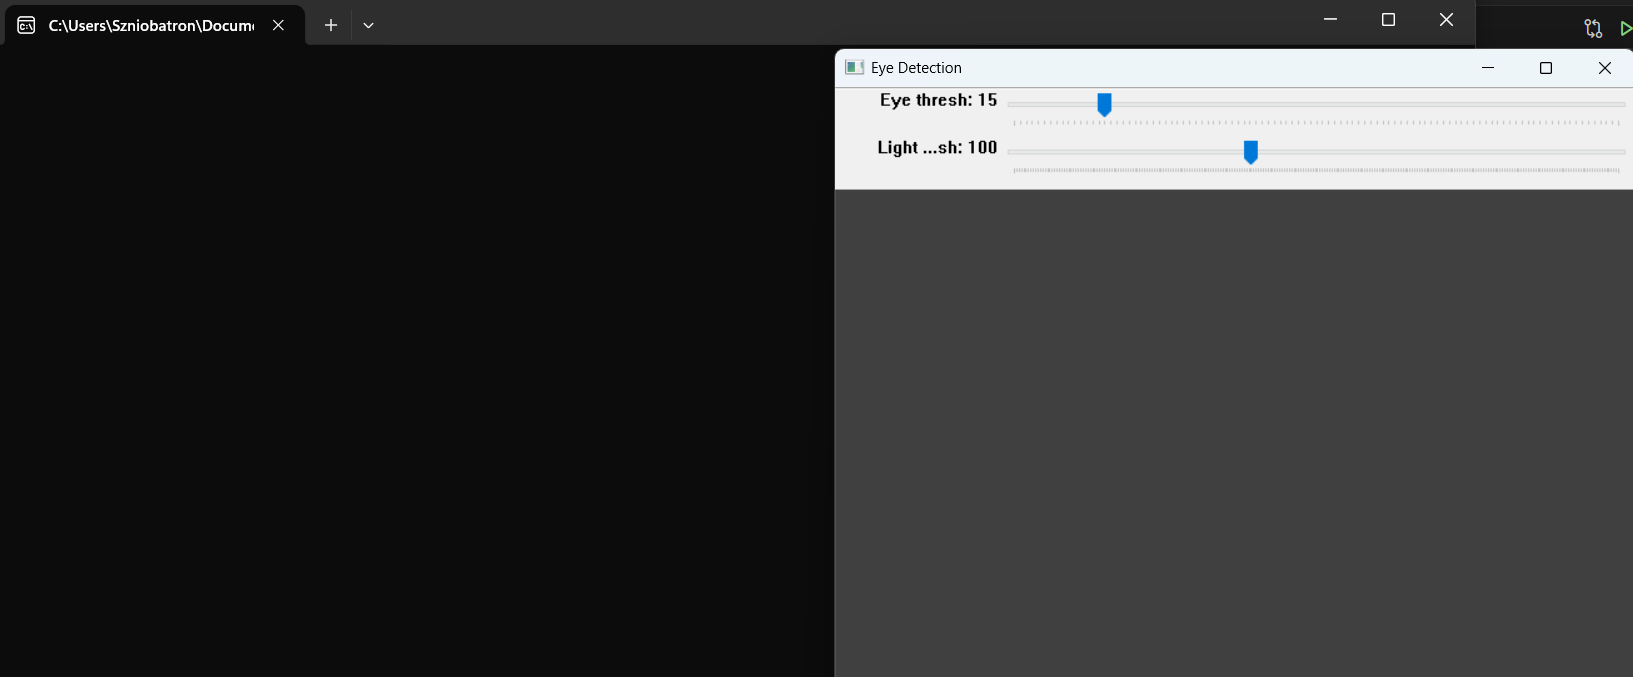
\includegraphics[width=0.6\textwidth]{pic/obsługa/okna przy otwarciu.png}
	\caption{Główne okna programu \texttt{eye\_\-detect.exe} w momencie uruchamiania, przed połączeniem z kamerą.}
	\label{fig:eye_detect-uruchamianie}
\end{figure}

Jeśli program uzyska dostęp do kamery automatycznie zacznie pobierać z niej obraz, który przekształci do odcieni szarości, żeby móc wyszukiwać na nim twarz i oczy używając klasyfikatora Haara. Gdy uda się wyszukać oczy, obraz w odcieniach szarości zostanie zbinaryzowany i poddany operacją morfologicznym w celu wyszukania źrenic. Wszystkie wykryte elementy zostają oznaczone na obrazie barwnym i wyświetlone w oknie ,,eye detection''. Podczas działania programu mogą otworzyć się jeszcze dwa dodatkowe okna: ,,Bin eyes for testing'', pojawiający się w momencie wykrycia oczu oraz ,,Bin reflection for testing'', które otworzy się w momencie włączenia trybu kalibracji zaawansowanej. ,,Bin eyes for testing'' obrazuje binaryzację źrenic przed (po lewej) i po (po prawej) operacjach morfologicznych, z kolei ,,Bin reflection for testing'' pokazuje binaryzację dla odbicia rogówkowego. Okna te są wizualizacją techniczną ułatwiającą dostrojenie programu i są przedstawione na rysunku \ref{fig:eye_detect-okna-bin}.

\begin{figure}[htbp]
	\centering
	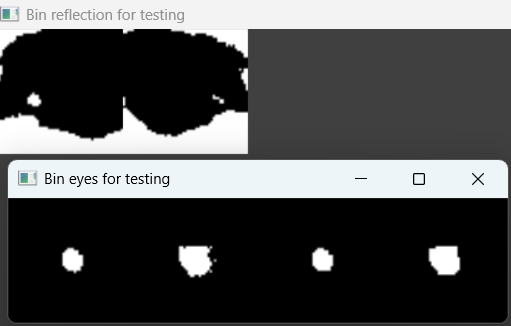
\includegraphics[width=0.6\textwidth]{pic/obsługa/okna binarne.png}
	\caption{Wizualizacja obrazów binarnych wykorzystywanych w procesie wykrywania źrenic i odbicia rogówkowego.}
	\label{fig:eye_detect-okna-bin}
\end{figure}

Użytkownik może wchodzić w interakcję z systemem na dwa sposoby, poprzez interfejs graficzny w formie suwaków widocznych na rysunku \ref{fig:eye_detect-uruchamianie}, lub przez naciśnięcie odpowiedniego klawisza na klawiaturze. Nad obrazem w oknie ,,eye detection'' widnieją dwa suwaki, których pozycje można zmieniać poprzez kliknięcie lub przeciąganie myszą. Suwak ,,Eye tresh'' (pierwszy od góry), odpowiada progowi używanego w binaryzacji źrenic, a jego wartość ustawiona jest na $15$, pozwalając na stabilne śledzenie przy dobrym oświetleniu frontalnym. Jednakże, w zależności od warunków oświetleniowych, a także preferencji związanych z stabilnością i dokładnością pomiaru, użytkownik powinien ręcznie dostosować wartość progu, aby zapewnić optymalną detekcję źrenic. Następny suwak ,,Light tresh'' (drugi od góry), używany jest jedynie w przypadku kalibracji zaawansowanej, on także odpowiada progowi binaryzacji, ale w tym przypadku odbicia rogówkowego. Użytkownik wyposażony w odpowiednio intensywne źródło światła i decydujący się na tego typu kalibrację punktu odniesienia, powinien ręcznie wybrać wartość na suwaku tak, aby na obrazie binaryzacji pozostał jedynie niewielki jasny punkt. 

Reszta funkcjonalności dostępna jest po naciśnięciu danego klawiszu na klawiaturze, ich wykaz prezentuje się następująco:

\begin{description}
	\item[z (kalibracja automatyczna) --] tryb kalibracji punktu odniesienia, który ustawiany jest w momencie uruchomienia programu. Pozwala na pomiar ruchu źrenic względem środka obszaru wykrytego oka.
	\item[x (kalibracja zaawansowana) --] tryb kalibracji punktu odniesienia na podstawie obrazu binarnego oka. Pozwala na pomiar ruchu źrenic względem wykrytego odbicia rogówkowego.
	\item[c (kalibracja ręczna) --]  tryb kalibracji punktu odniesienia na aktualną pozycję źrenic. Pozwala na pomiar ruchu źrenic względem ustalonego miejsca w obszarze wykrytego oka.
	\item[r (przełączanie trybów rysowania) --] są dostępne trzy tryby rysowania wykrytych obszarów na obrazie z kamery. Pierwszy tryb jest ustawiony wraz z uruchomieniem programu obrysowując: twarz, ograniczony obszar twarzy, oczy, źrenice, środki źrenic oraz punkt odniesienia. Drugi tryb pozwala na większą przejrzystość rysując najistotniejsze elementy detekcji, czyli środek źrenic i punkt odniesienia. Trzeci tryb wyłącza rysowanie, zwracając niezmodyfikowany obraz z kamery.
	\item[q (wyłączenie programu) --] jedyny poprawny sposób na zatrzymanie systemu, po naciśnięciu bezpiecznie zamyka plik tekstowy z pomiarami, zwalnia kamerę i zamyka wszystkie okna programu.
\end{description}

Po udanej sesji śledzenia ruchu gałek ocznych, można zwizualizować zebrane pomiary zapisane w pliku tekstowym, otwierając plik \texttt{eye\_\-tracking\_\-plot.exe} umieszczony w tym samym folderze co plik tekstowy. Wygenerowane zostaną trzy zestawy wykresów w osobnych oknach, przedstawiając przemieszczenie źrenicy w osi względem punktu odniesienia (dla obu oczu wspólnie i osobno). Zostały one utworzone przy pomocy Pyplot, pozwalając użytkownikowi na swobodne przybliżanie i poruszanie się po wykresach. Możliwe jest także zapisanie utworzonego wykresu w wielu popularnych rozszerzeniach. Okna z wykresami wraz z terminalem przedstawione są na rysunku \ref{fig:eye_tracking_plot-wykresy-i-terminal}.

\begin{figure}[htbp]
	\centering
	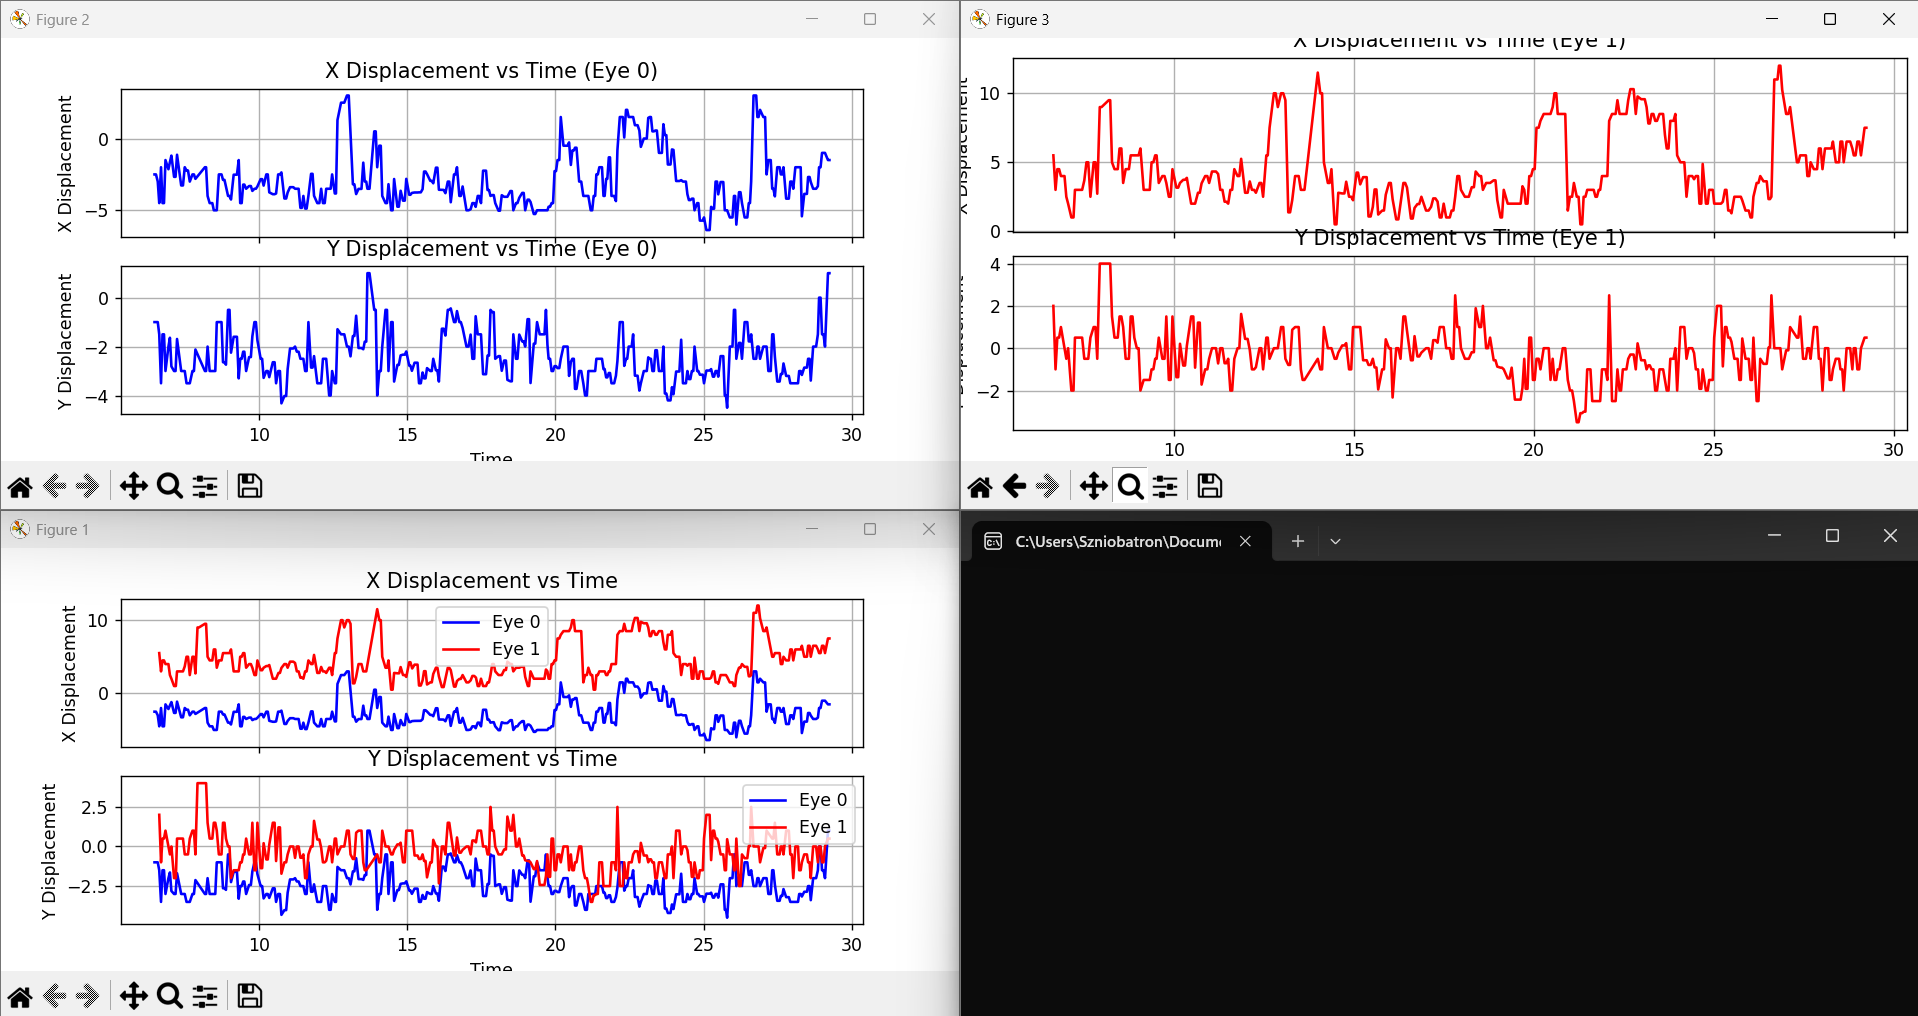
\includegraphics[width=0.6\textwidth]{pic/obsługa/wykresy.png}
	\caption{Okna programu \texttt{eye\_\-tracking\_\-plot.exe}, przedstawiające wykresy czasowe przemieszczenia źrenicy i terminal.}
	\label{fig:eye_tracking_plot-wykresy-i-terminal}
\end{figure}

W momencie zamknięcia programu, wszystkie okna, a w tym okno terminalu, zostają zamknięte. Z racji tego, użytkownicy zainteresowani informacjami zwracanymi w terminalu -- takimi jak informacja o błędzie, które mogą zostać zwrócone w przypadku uszkodzonego pliku, lub braku dostępu do kamery -- mogą uruchomić dany plik przy użyciu terminala. Wystarczy ustawić katalog roboczy terminala na ten, w którym znajduje się plik wykonywalny, a następnie wpisać jego nazwę wraz z rozszerzeniem i nacisnąć enter. W ten sposób po zakończeniu działania programu informacje w terminalu zostaną zachowane.

\section{Kwestie bezpieczeństwa}
\label{sec:Kwestie-bezpieczenstwa}

System do śledzenia ruchu gałek ocznych w żaden sposób nie przechowuje oraz nie nagrywa obrazów z kamery komputera, a wszelkie wykorzystywane zasoby zostają zwolnione w momencie zakończenia działania. Jedyną zapisywaną informacją są pomiary w pliku tekstowym, dostępnym w tym samym folderze co plik \texttt{eye\_\-detect.exe}, które można z łatwością usunąć przenosząc do kosza, a następnie opróżniając go. Prezentowany program nie korzysta także z połączenia sieciowego, wykonując wszystkie operacje lokalnie w katalogu, w którym się znajduje. 

PyInstaller ostrzega, że istnieją niebezpieczeństwa związane z używaniem plików wykonywalnych w formie jednego pliku. PyInstaller rozpakowuje część swoich zasobów do tymczasowego folderu (nazwy zaczynające się od \_MEI) podczas uruchamiania aplikacji. Jeśli program zostanie nieoczekiwanie przerwany np. przez awarię, lub zakończenie przez Menedżera Zadań, folder ten może nie zostać usunięty. W skrajnych przypadkach -- przy częstych awariach -- może dojść do gromadzenia się niepotrzebnych plików, co w długoterminowej perspektywie może zużywać miejsce na dysku. Możliwe jest ręczne usunięcie nadmiarowych plików, które w przypadku systemu Windows zazwyczaj znajdują się w folderze ,,Temp'', można wyszukać jego lokalizację wpisując komendę \texttt{ECHO \-\%Temp\%} w wierszu poleceń. Nie należy także otwierać plików wykonywalnych utworzonych przez PyInstaller z uprawnieniami administratora, ponieważ daje to teoretyczną możliwość, że atakujący mógłby modyfikować pliki w tymczasowym folderze. Taka modyfikacja mogłaby potencjalnie prowadzić do eskalacji uprawnień \cite{bib:PyInstaller-how-it-works}.

\section{Scenariusze korzystania z systemu}
\label{Scenariusze-korzystania-z-systemu}

Dla lepszego zobrazowania możliwości systemu śledzącego ruch gałek ocznych przedstawione zostaną kroki przykładowego scenariusza, ilustrowany zrzutami ekranu. 

\begin{enumerate}
	\item Użytkownik decyduje się na podjęcie śledzenia, więc uruchamia plik wykonywalny \texttt{eye\_\-detect.exe} (rysunek \ref{fig:scenariusz-odpalanie-sledzenia}).

	\begin{figure}[H]
		\centering
		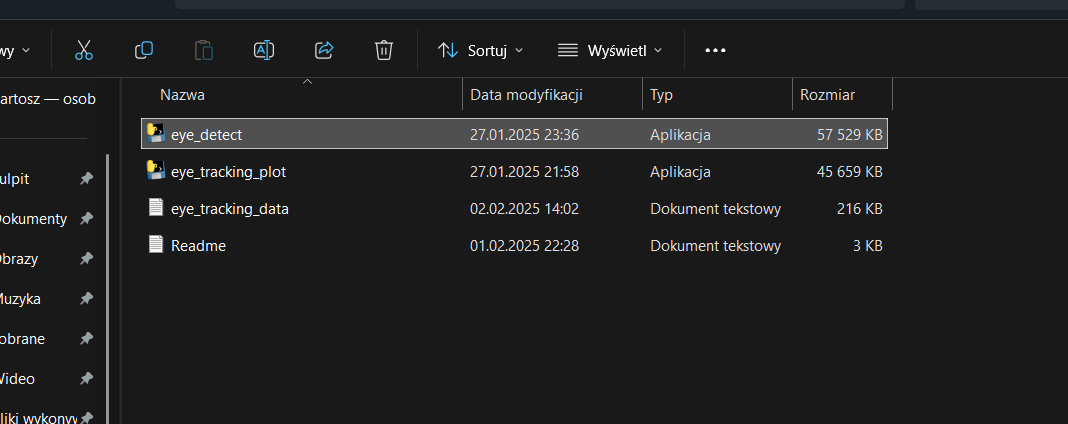
\includegraphics[width=0.6\textwidth]{pic/scenariusz/odpalamy śledzenie.png}
		\caption{Użytkownik decyduje się na rozpoczęcie śledzenia.}
		\label{fig:scenariusz-odpalanie-sledzenia}
	\end{figure}

	\item Program nie napotkał żadnych błędów i uruchomił się poprawnie wyświetlając obraz z kamery, źrenice nie zostały wykryte z powodu niesprzyjającego oświetlenia (rysunek \ref{fig:scenariusz-siema}).
	
	\begin{figure}[H]
		\centering
		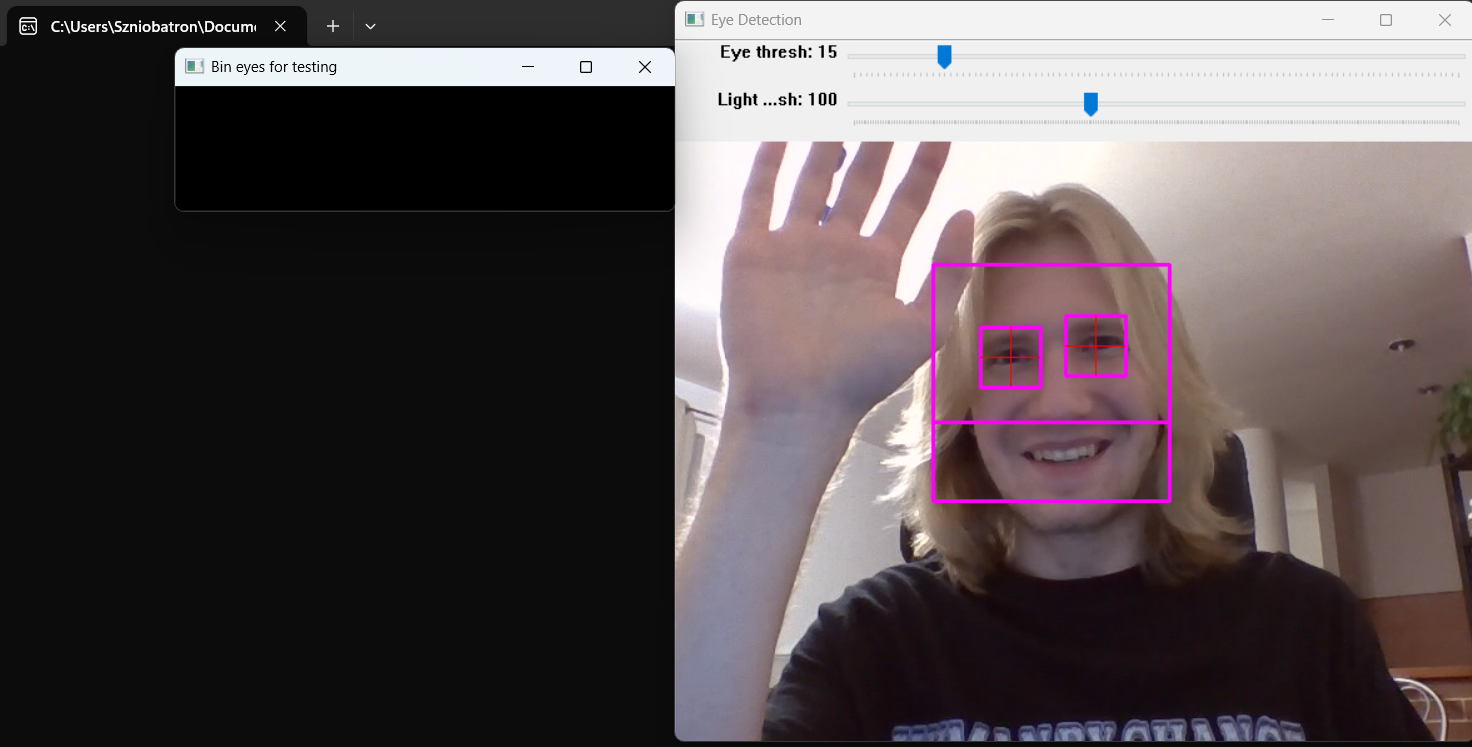
\includegraphics[width=0.6\textwidth]{pic/scenariusz/śledzenie start.png}
		\caption{Użytkownik uruchomił pomyślnie system do śledzenia ruchu gałek ocznych.}
		\label{fig:scenariusz-siema}
	\end{figure}

	\item Użytkownik poprawił swoje otoczenie, oświetlając twarz od frontu i odsłaniając włosy, tak żeby nie przeszkadzały w detekcji. Zmieniono także ustawienia, zwiększając próg detekcji i kalibrując punkt odniesienia przez spojrzenie się na środek ekranu i naciśnięcie klawisz ,,c'' (rysunek \ref{fig:scenariusz-poprawione-swiatlo}).
	
	\begin{figure}[H]
		\centering
		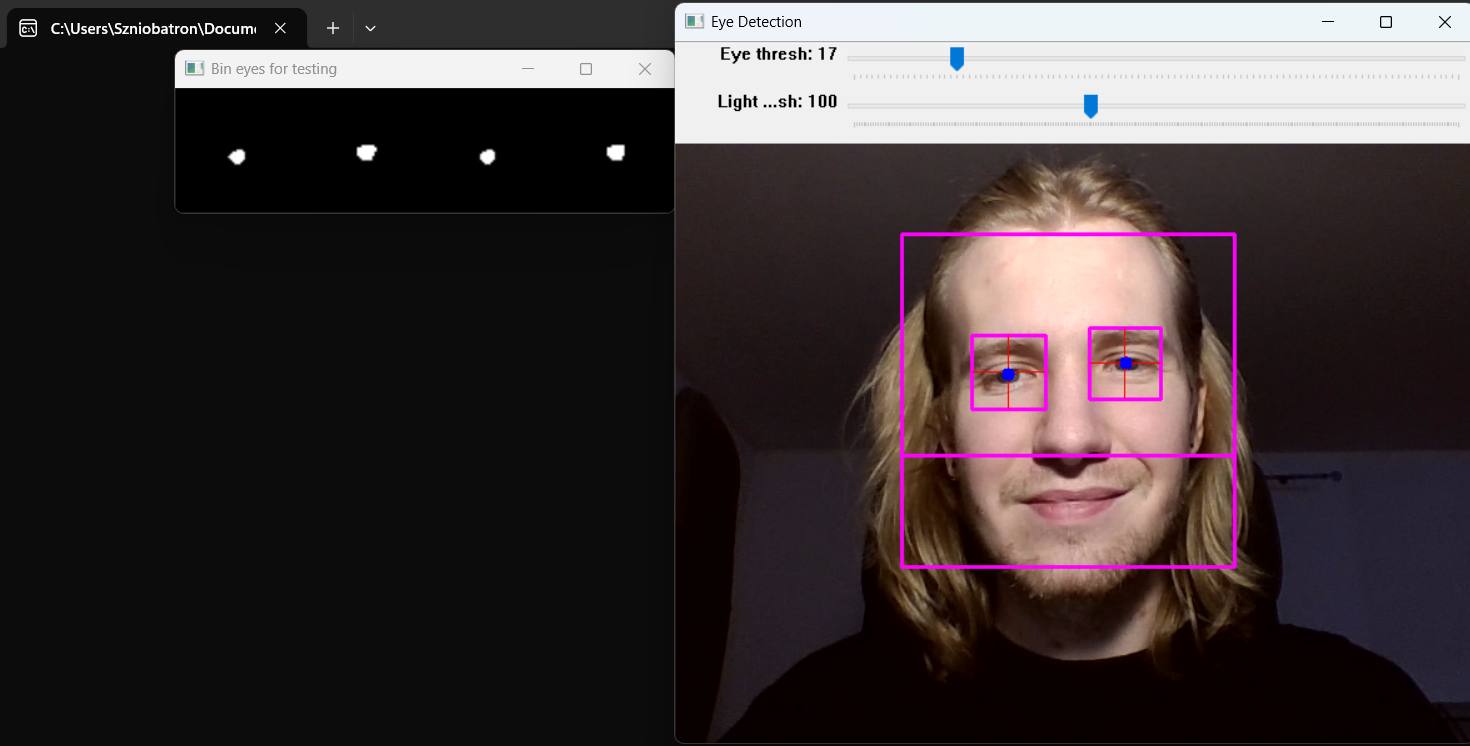
\includegraphics[width=0.6\textwidth]{pic/scenariusz/poprawienie śledzenia.png}
		\caption{Użytkownik poprawił warunki oświetleniowe i dostosował ustawienia programu.}
		\label{fig:scenariusz-poprawione-swiatlo}
	\end{figure}

	\item Celem śledzenia była analiza ruchu gałek ocznych w trakcie oglądania krótkiego filmu na platformie YouTube (rysunek \ref{fig:scenariusz-yt}) \cite{bib:youtube}.
	
	\begin{figure}[H]
		\centering
		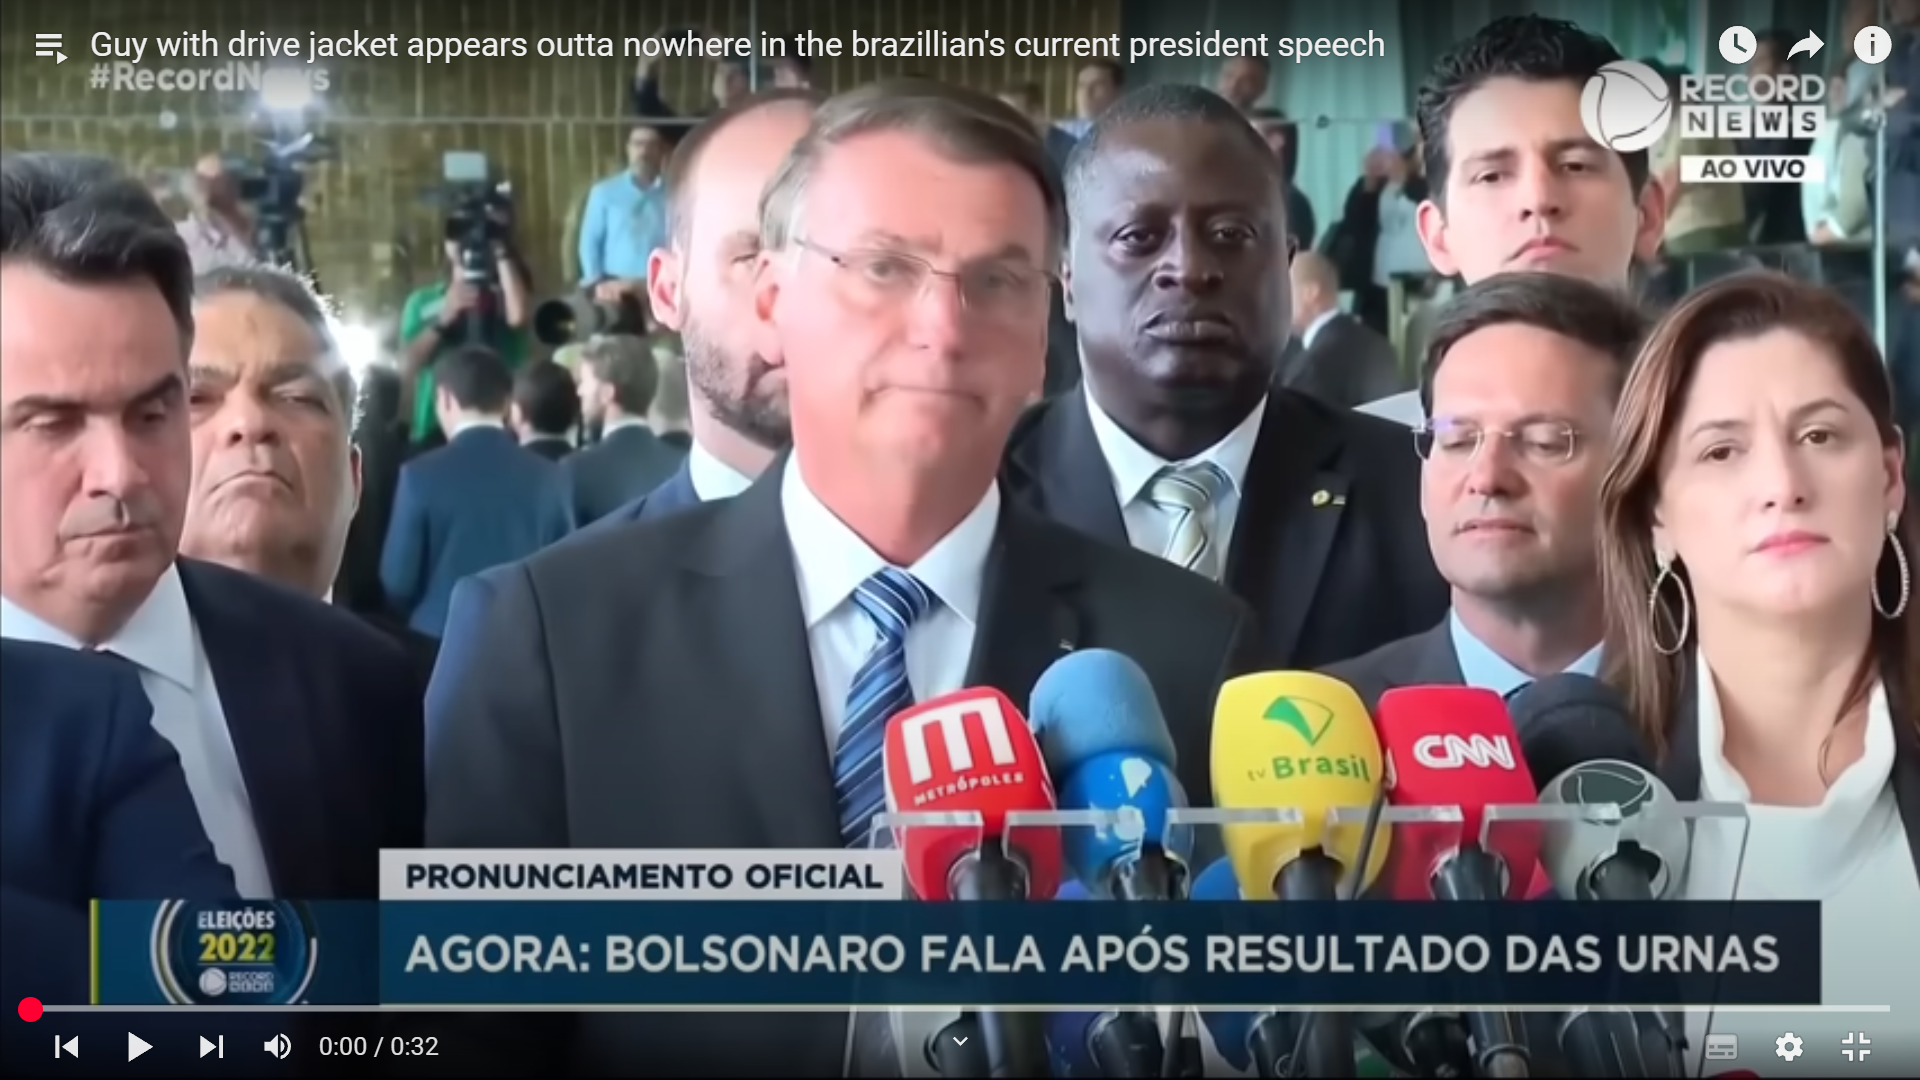
\includegraphics[width=0.6\textwidth]{pic/scenariusz/filmik yt.png}
		\caption{Użytkownik uruchamia krótkie nagranie do analizy uwagi wzrokowej.}
		\label{fig:scenariusz-yt}
	\end{figure}

	\item Po przeprowadzonym eksperymencie naciśnięto klawisz ,,q'' zakańczając pomiar. Użytkownik następnie zdecydował się na wygenerowanie wykresów czasowych do analizy i uruchomił plik \texttt{eye\_\-tracking\_\-plot.exe} (rysunek \ref{fig:scenariusz-odpalanie-wykresy}).
	
	\begin{figure}[H]
		\centering
		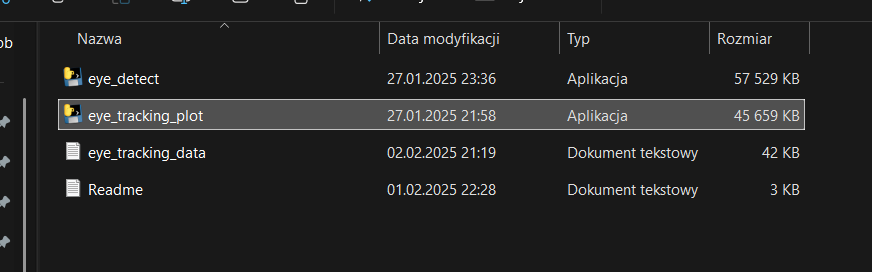
\includegraphics[width=0.6\textwidth]{pic/scenariusz/odpalam wykresy.png}
		\caption{Użytkownik decyduje się na wygenerowanie wykresów czasowych z zebranych pomiarów.}
		\label{fig:scenariusz-odpalanie-wykresy}
	\end{figure}

	\item Analiza zebranych pomiarów w tym przypadku najlepiej widoczna jest dla wykresów obu oczu jednocześnie. Filmik trwał $33$ sekundy, a spojrzenie kierowane było głównie na środek ekranu i wzdłuż osi $Y$, co widoczne jest na wykresie (rysunek \ref{fig:scenariusz-analiza-wykresy}).
	
	\begin{figure}[H]
		\centering
		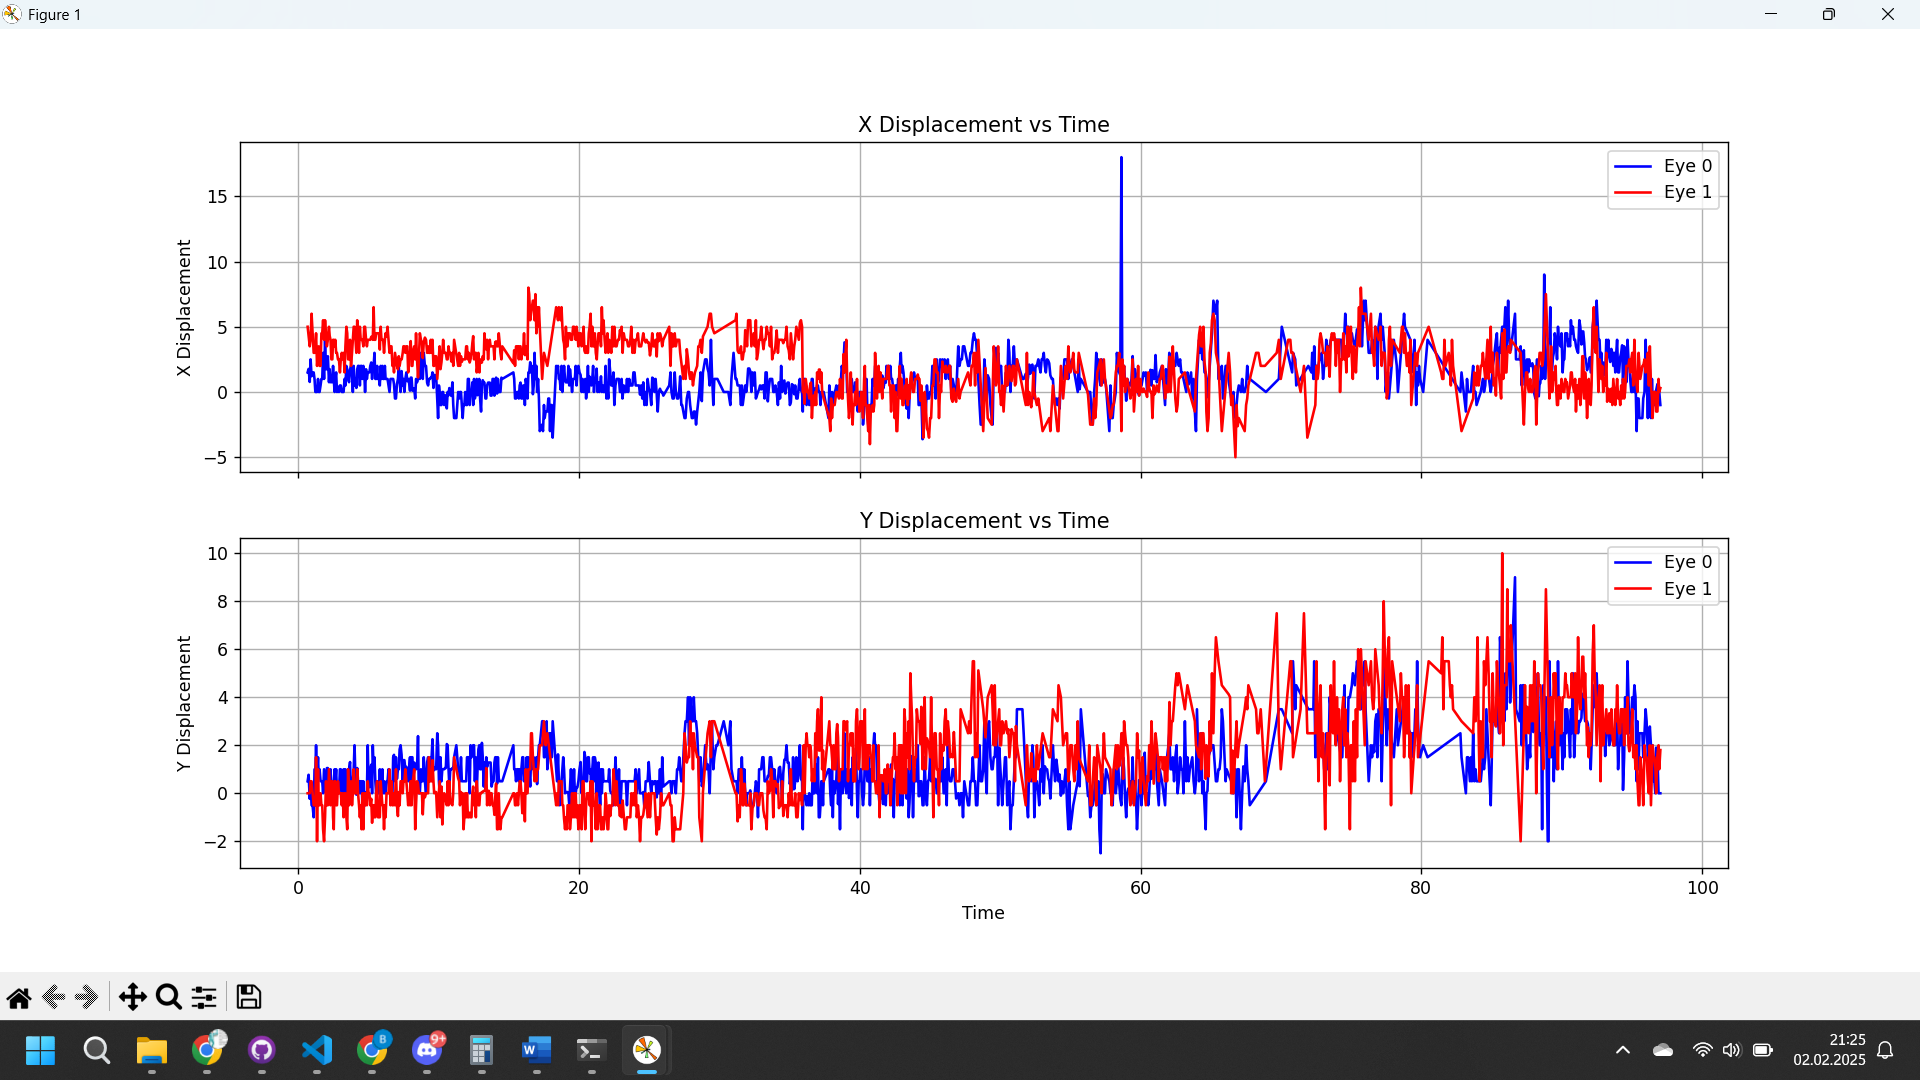
\includegraphics[width=0.6\textwidth]{pic/scenariusz/analiza wykresów.png}
		\caption{Użytkownik analizuje wykresy dla obu oczu.}
		\label{fig:scenariusz-analiza-wykresy}
	\end{figure}

	\item Użytkownik przybliżył wykresy na interesującą część, a następnie zmodyfikował rozmieszczenie i wielkość pola wykresów, dla lepszej widoczności (rysunek \ref{fig:scenariusz-ustawianie-wykresy}).
	
	\begin{figure}[H]
		\centering
		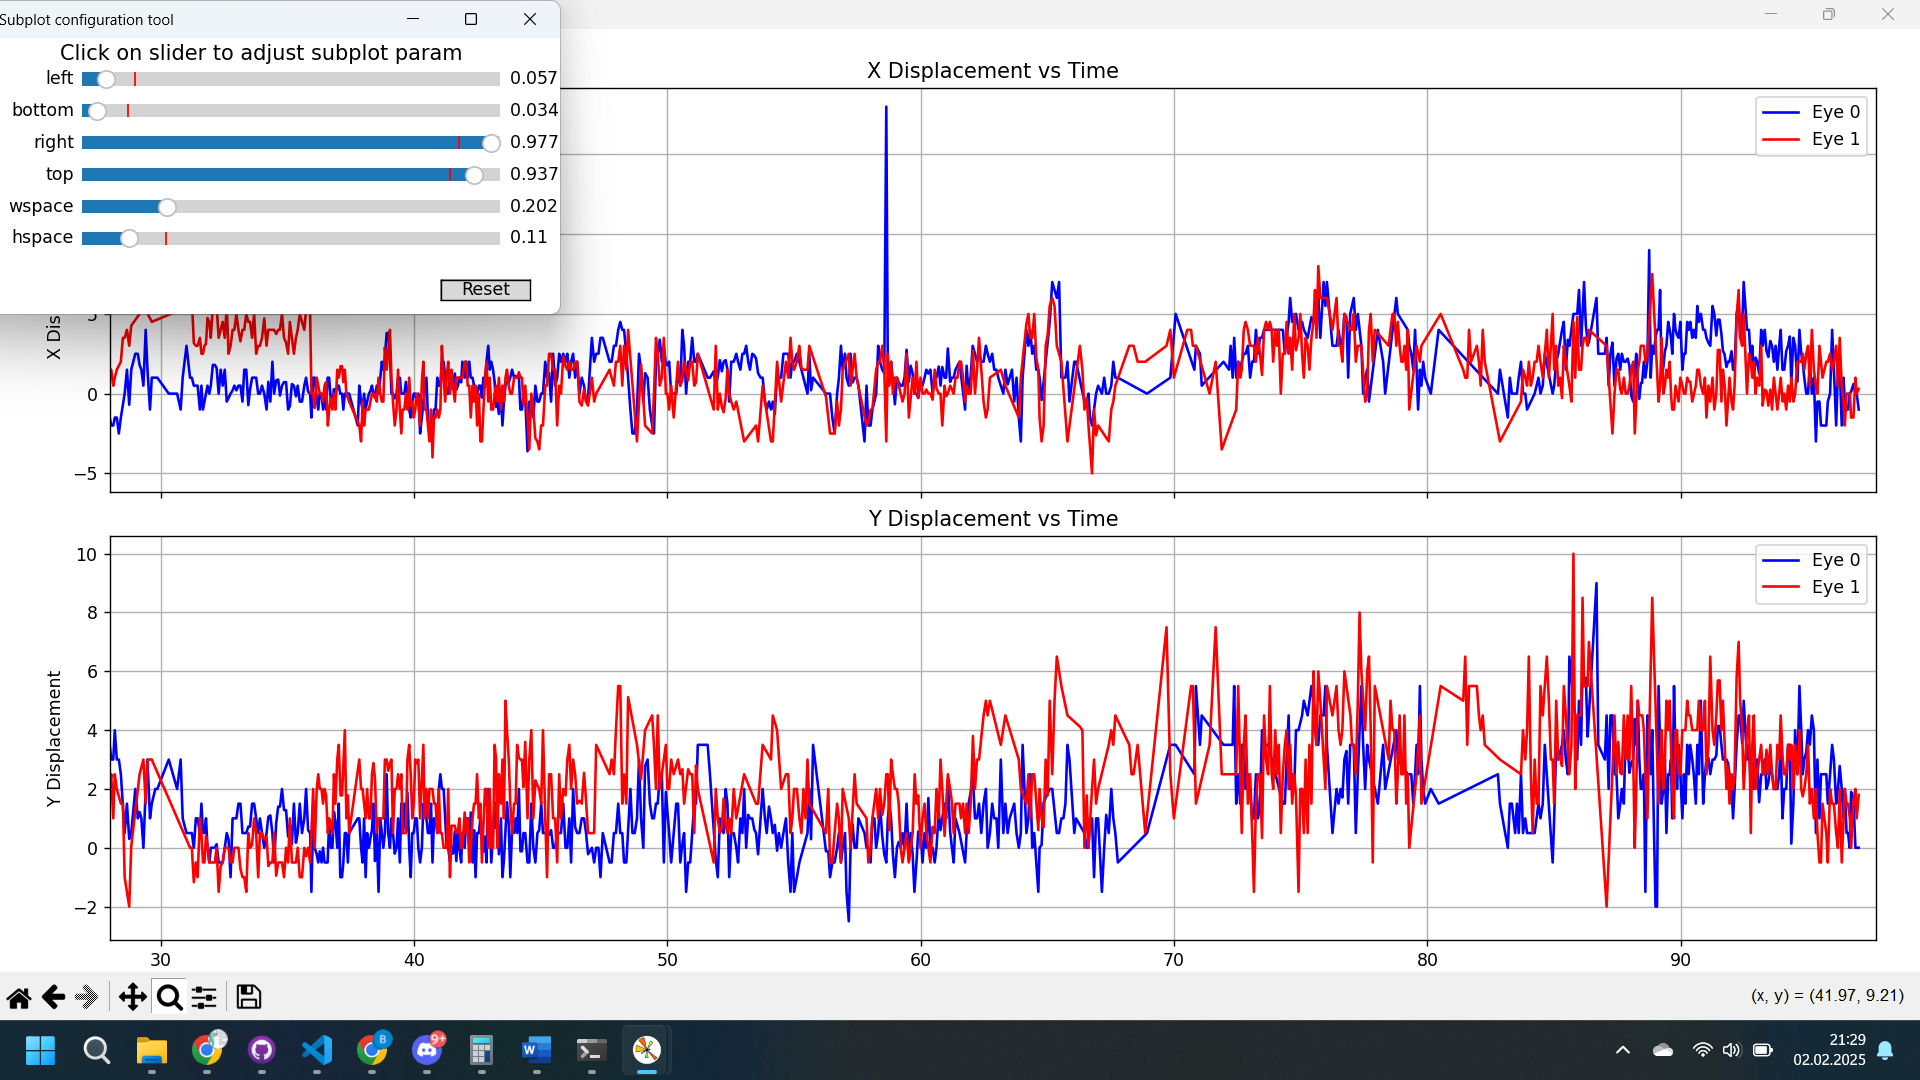
\includegraphics[width=0.6\textwidth]{pic/scenariusz/dostosowanie wykresów.png}
		\caption{Użytkownik dostosowuje ustawienia wizualne wykresów.}
		\label{fig:scenariusz-ustawianie-wykresy}
	\end{figure}

	\item Na koniec wykresy zostają zapisane, użytkownik może wybrać format, który najbardziej odpowiada jego wymaganiom i preferencją (rysunek \ref{fig:scenariusz-zapisywanie-wykresy})
	
	\begin{figure}[H]
		\centering
		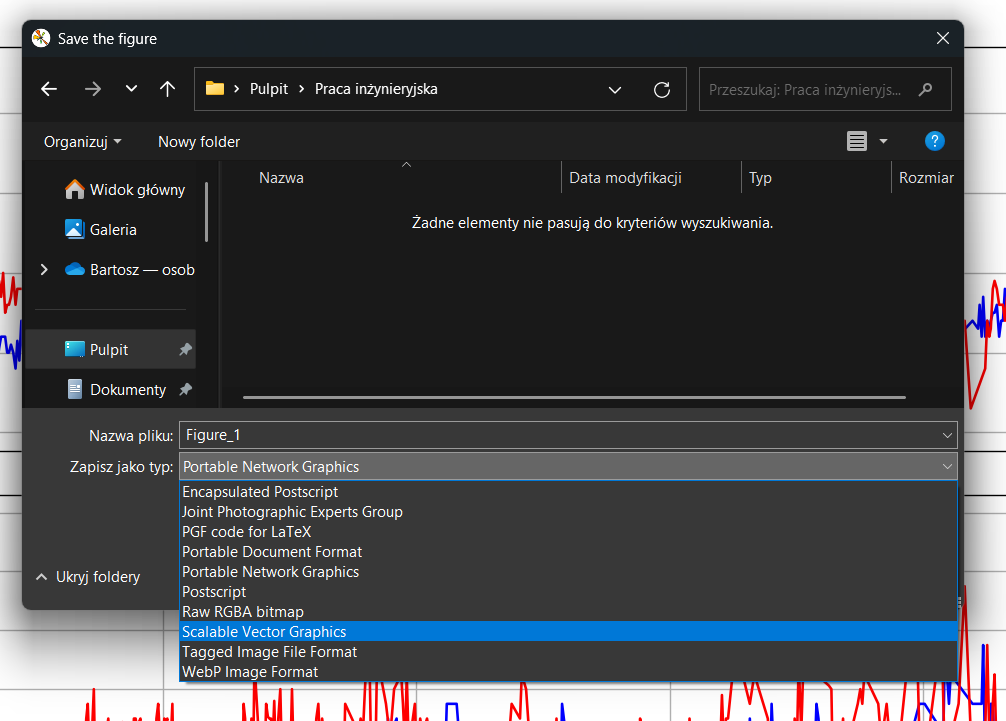
\includegraphics[width=0.6\textwidth]{pic/scenariusz/zapisanie wykresow.png}
		\caption{Użytkownik zapisuje wykresy czasowe w wybranym przez siebie rozszerzeniu.}
		\label{fig:scenariusz-zapisywanie-wykresy}
	\end{figure}
\end{enumerate}

Jeśli „Specyfikacja zewnętrzna”:
\begin{itemize}
\item  wymagania sprzętowe i programowe
\item  sposób instalacji
\item  sposób aktywacji
\item  kategorie użytkowników
\item  sposób obsługi
\item  administracja systemem
\item  kwestie bezpieczeństwa
\item  przykład działania
\item  scenariusze korzystania z systemu (ilustrowane zrzutami z ekranu lub generowanymi dokumentami)
\end{itemize}

%%%%%%%%%%%%%%%%%%%%%
%% RYSUNEK Z PLIKU
%
%\begin{figure}
%\centering
%
\includegraphics[width=0.5\textwidth]{./politechnika_sl_logo_bw_pion_pl.pdf}
%\caption{Podpis rysunku zawsze pod rysunkiem.}
%\label{fig:etykieta-rysunku}
%\end{figure}
%Rys. \ref{fig:etykieta-rysunku} przestawia …
%%%%%%%%%%%%%%%%%%%%%
%
%%%%%%%%%%%%%%%%%%%%%
%% WIELE RYSUNKÓW 
%
%\begin{figure}
%\centering
%\begin{subfigure}{0.4\textwidth}
%    
\includegraphics[width=\textwidth]{./politechnika_sl_logo_bw_pion_pl.pdf}
%    \caption{Lewy górny rysunek.}
%    \label{fig:lewy-gorny}
%\end{subfigure}
%\hfill
%\begin{subfigure}{0.4\textwidth}
%    
\includegraphics[width=\textwidth]{./politechnika_sl_logo_bw_pion_pl.pdf}
%    \caption{Prawy górny rysunek.}
%    \label{fig:prawy-gorny}
%\end{subfigure}
%
%\begin{subfigure}{0.4\textwidth}
%    
\includegraphics[width=\textwidth]{./politechnika_sl_logo_bw_pion_pl.pdf}
%    \caption{Lewy dolny rysunek.}
%    \label{fig:lewy-dolny}
%\end{subfigure}
%\hfill
%\begin{subfigure}{0.4\textwidth}
%    
\includegraphics[width=\textwidth]{./politechnika_sl_logo_bw_pion_pl.pdf}
%    \caption{Prawy dolny rysunek.}
%    \label{fig:prawy-dolny}
%\end{subfigure}
%        
%\caption{Wspólny podpis kilku rysunków.}
%\label{fig:wiele-rysunkow}
%\end{figure}
%Rys. \ref{fig:wiele-rysunkow} przestawia wiele ważnych informacji, np. rys. \ref{fig:prawy-gorny} jest na prawo u góry.
%%%%%%%%%%%%%%%%%%%%%


 
\begin{figure}
\centering
\begin{tikzpicture}
\begin{axis}[
    y tick label style={
        /pgf/number format/.cd,
            fixed,   % po zakomentowaniu os rzednych jest indeksowana wykladniczo
            fixed zerofill, % 1.0 zamiast 1
            precision=1,
        /tikz/.cd
    },
    x tick label style={
        /pgf/number format/.cd,
            fixed,
            fixed zerofill,
            precision=2,
        /tikz/.cd
    }
]
\addplot [domain=0.0:0.1] {rnd};
\end{axis} 
\end{tikzpicture}
\caption{Podpis rysunku po rysunkiem.}
\label{fig:22}
\end{figure}



%--------------------------------------
%
%
% TODO:  przegląd ważniejszych algorytmów (jeśli występują), szczegóły implementacji wybranych fragmentów
%
% Status: 7s0%
%--------------------------------------
\chapter{Specyfikacja wewnętrzna}
\label{ch:Specyfikacja-wewnetrzna}

\section{Przedstawienie idei}
\label{sec:Przedstawienie-idei}

Z powodu architektury programu \texttt{eye\-\_detect.exe} zrozumienie jego idei opisanej jedynie słownie może okazać się wyzwaniem, dlatego stworzono diagram aktywności, który obrazuje wszystkie możliwe ścieżki działania programu w jednolity sposób. Niestety nawet taka forma opisu, chociaż bardziej przejrzysta, wciąż jest bardzo obszerna, w związku z tym diagram podzielony został na cztery osobne rysunki (rysunek \ref{fig:diagram-aktywnosci-1}, \ref{fig:diagram-aktywnosci-2}, \ref{fig:diagram-aktywnosci-3} i \ref{fig:diagram-aktywnosci-4}), które należy rozumieć jako jedną całość. Rozwiązanie te można podzielić na kilka części. 

Inicjalizacja to część programu wykonująca się tylko raz na jego początku tworząc podstawowy interfejs oraz zmienne, w tym do przechowywania informacji dla obu oczu. Otwierany jest także plik tekstowy do zapisu pomiarów, w którym zapisywany jest nagłówek. W tej części jest także kontrola błędu sprawdzająca poprawność załadowania klasyfikatorów Haara i połączenia z kamerą. Następnie program wchodzi w główną nieskończoną pętle, to w niej wykonywane są wszystkie funkcje systemu. W pętli tej pobierana jest klatka z kamery, na której następnie wykrywane są wszystkie możliwe twarze i oczy kaskadą Haara, w zależności od sposobu kalibracji wyznaczany jest także punkt odniesienia, następnie wykrywane są źrenice przez binaryzację i operacje morfologiczne obrazu w odcieniach szarości. Gdy wyznaczenie punktu odniesienia i środka źrenicy się powiodło, program oblicza przesunięcie względem nich w osi $X$ i $Y$, a następnie zapisuje pomiar z indeksem oka i momentem czasowym do pliku tekstowego. W przypadku niepowodzenia na jednym z etapów detekcji, system po prostu przechodzi dalej, czekając na zmianę. W trakcie wykonywania się pętli program sprawdza spełnienie warunków by ustalić sposób kalibracji, a także tryb rysowania determinujacy sposób oznaczania wykrytych elementów. Na koniec wyświetlany jest obraz z kamery po wszystkich modyfikacjach, a także sprawdzane jest wprowadzenie przycisku z klawiatury, które może zmienić wartości zmiennych determinując sposób rysowania i kalibracji. Jeśli użytkownik naciśnie klawisz ,,q'' pętla zostaje przerwana, zasób kamery zostaje zwolniony, plik tekstowy zostaje bezpiecznie zamkniety i wszystkie okna zostają zniszczone, zakańczając działanie \texttt{eye\-\_detect.exe}. 

Program \texttt{eye\_\-tracking\_\-plot.exe} ze względu na nieskomplikowanie nie posiada diagramu aktywności. Wpierw odczytywany jest plik \texttt{eye\_tracking\_data.txt} z oznaczeniem separatora danych. Następnie wykreślane są trzy wykresy złożone, za każdym razem w analogiczny sposób z użyciem funkcji biblioteki \texttt{Matplotlib\-.pyplot}: ustalany jest rozmiar wykresów i współdzielenie osi $X$; program przechodzi przez wszystkie dane w pliku, grupuje indeksami i ustala wartość na osiach; na wykres nanoszone są punkty, które łączone są prostą linią o odpowiednim kolorze; ustalane zostają ustawienia wykresów, takie jak nazwy osi, tytuły i obecność siatki. Program przeprowadza te operacje dla każdego wykresu złożonego, który prezentowany jest w osobnych oknach, dzięki temu wyświetlone zostają wykresy przemieszczenia w obu osiach, dla każdego oka z osobna oraz wspólnie.

\begin{figure}[htbp]
	\centering
	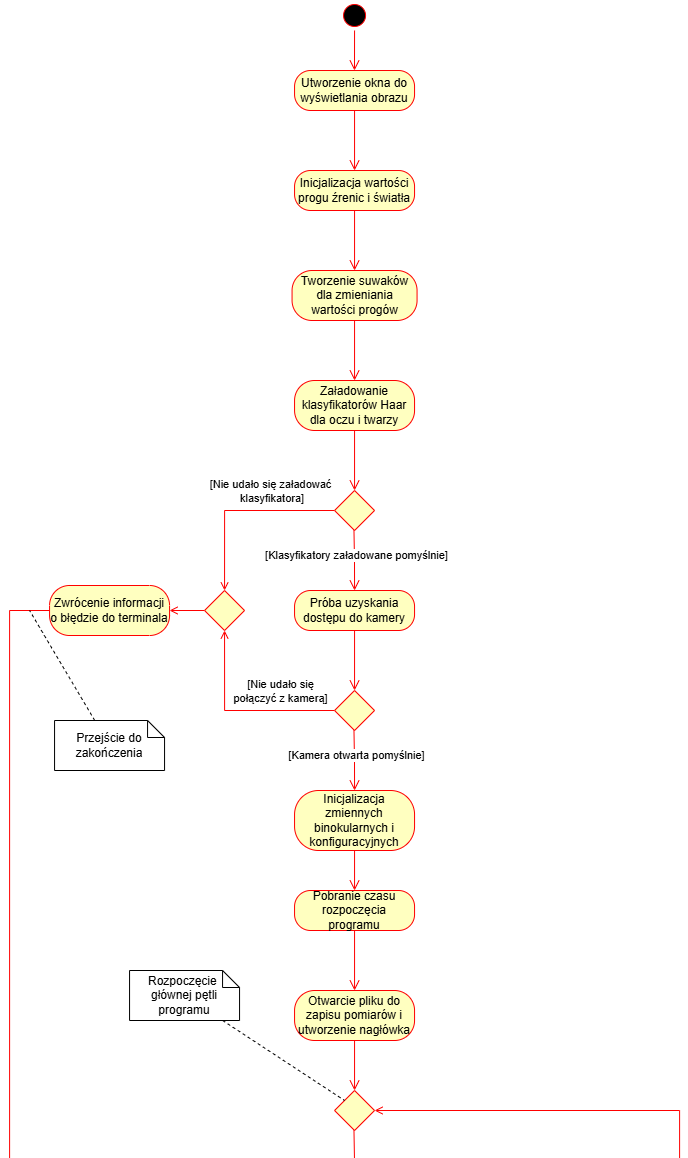
\includegraphics[width=0.6\textwidth, height=0.96\textheight]{pic/diagram aktywności/druga próba/diagram aktywności 1.png}
	\caption{Diagram aktywności programu \texttt{eye\-\_detect.exe} (część 1).}
	\label{fig:diagram-aktywnosci-1}
\end{figure}

\begin{figure}[htbp]
	\centering
	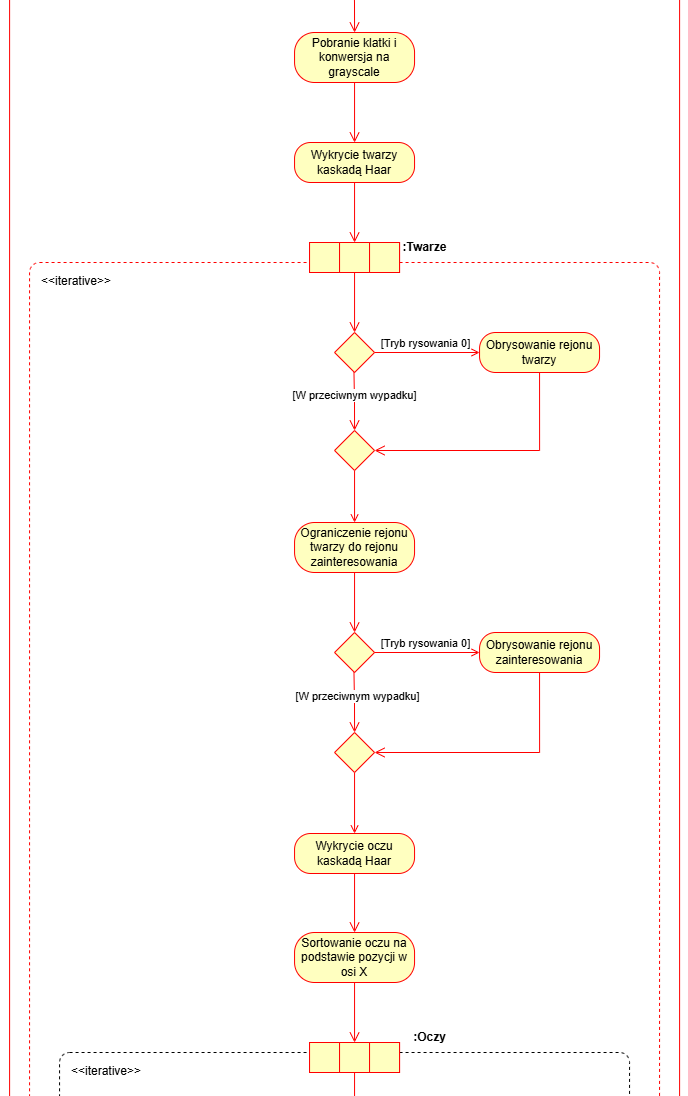
\includegraphics[width=0.6\textwidth, height=0.96\textheight]{pic/diagram aktywności/druga próba/diagram aktywności 2.png}
	\caption{Diagram aktywności programu \texttt{eye\-\_detect.exe} (część 2).}
	\label{fig:diagram-aktywnosci-2}
\end{figure}

\begin{figure}[htbp]
	\centering
	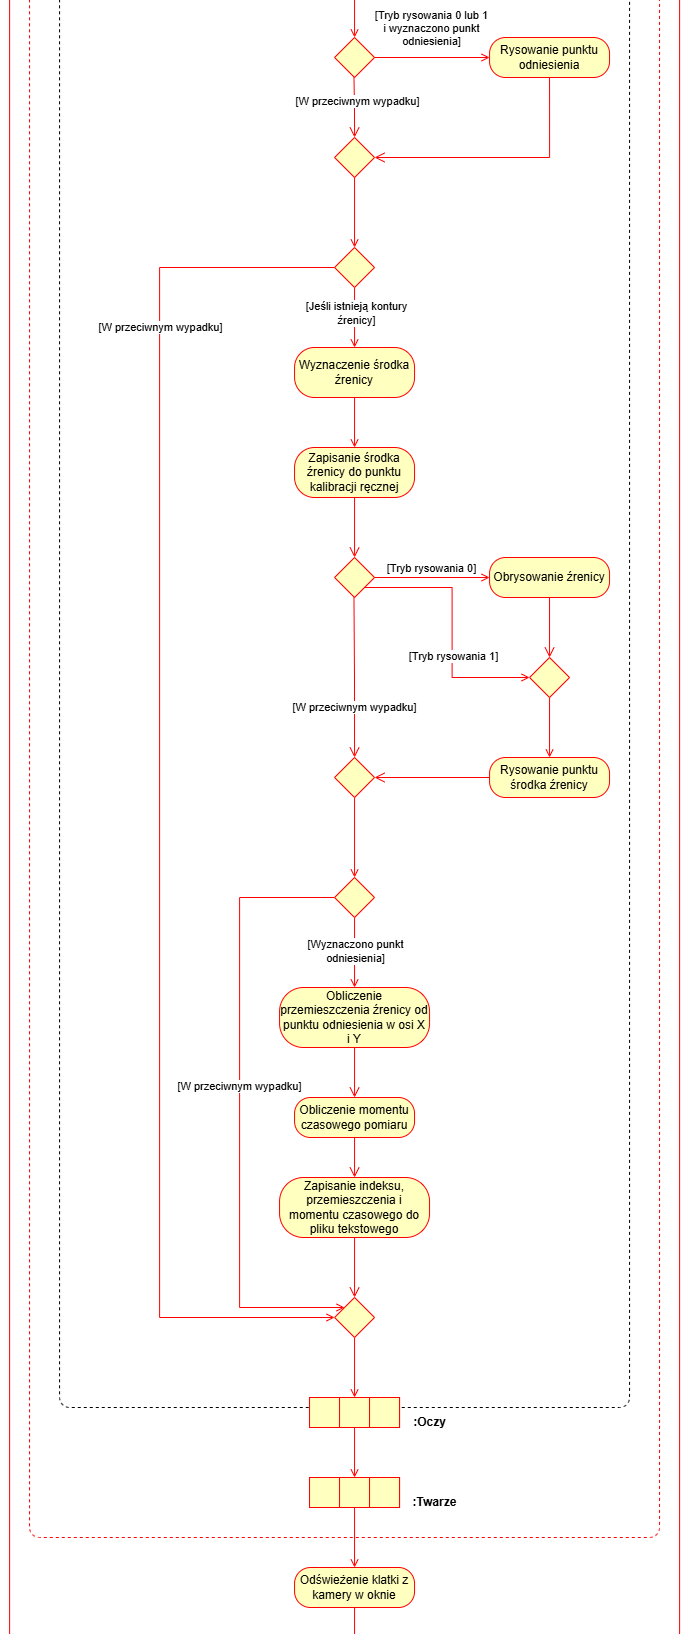
\includegraphics[width=0.6\textwidth]{pic/diagram aktywności/druga próba/diagram aktywności 3.png}
	\caption{Diagram aktywności programu \texttt{eye\-\_detect.exe} (część 3).}
	\label{fig:diagram-aktywnosci-3}
\end{figure}

\begin{figure}[htbp]
	\centering
	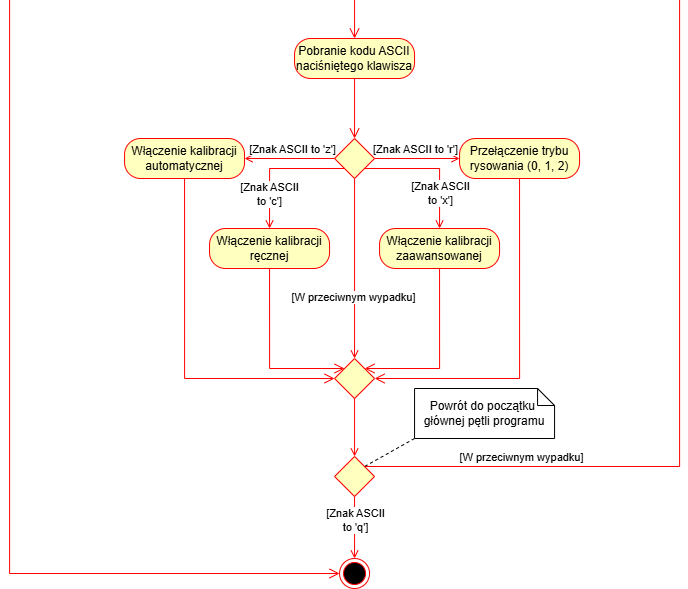
\includegraphics[width=0.6\textwidth]{pic/diagram aktywności/druga próba/diagram aktywności 4.png}
	\caption{Diagram aktywności programu \texttt{eye\-\_detect.exe} (część 4).}
	\label{fig:diagram-aktywnosci-4}
\end{figure}
\FloatBarrier

\section{Architektura systemu}
\label{sec:Architektura-systemu}

System wizyjny do śledzenia ruchu gałek ocznych opiera się na prostej architekturze, oba programy posiadają strukturę monolityczną. Struktura ta posiada jedną warstwę, w której realizowane są wszystkie funkcję programu, w przypadku \texttt{eye\_\-tracking\_\-plot.exe} wykonywane są tylko raz, a \texttt{eye\-\_detect.exe} wykonuje większość operacji w głównej pętli programu do momentu jej przerwania. Kod można opisać, że jest napisany w bardzo podstawowym paradygmacie imperatywnym, czyli takim, który operuje na ciągu instrukcji zmieniających stan programu, nie dzieląc go na własne obiekty, klasy czy struktury funkcji. Program zmienia swój stan przez sekwencyjne instrukcje, korzystając z pętli i warunków do określenie następnej ścieżki wykonywania. Kolejnym aspektem tego rozwiązania jest manipulacja zasobami komputera w sposób bezpośredni, zarówno względem pamięci komputera, używając zmiennych globalnych, jak i zasobów sprzętowych, łącząc się z kamerą i pobierając znaki ASCII z klawiatury. Nie dochodzi także do bezpośredniej komunikacji pomiędzy \texttt{eye\-\_detect.exe}, a \texttt{eye\_\-tracking\_\-plot.exe}, programy te są samodzielne i niezależne, ich jedynym elementem wspólnym jest wykorzystywanie pliku tekstowego \texttt{eye\_tracking\_data.txt} i to przez niego dochodzi do przekazania informacji.

\section{Opis struktur danych}
\label{sec:Opis-struktury-danych}

By móc omówić zapisywane dane, trzeba wpierw opisać jak system przechowuje wartości w zmiennych. Program \texttt{eye\-\_detect\-.exe} posiada między innymi zmienne będące instancjami klas bibliotek i zmienne pojedyncze, które przechowują wartości progów binaryzacji, czasu oraz stanów wykorzystywanych w warunkach. Jednakże większość zmiennych używanych w kodzie jest listami dwóch elementów, które przechowują wartości uporządkowane względem pozycji dla obu oczu. Program \texttt{eye\_\-tracking\_\-plot\-.exe} używa jedynie instancji klas przechowujących wartości pomiarów z pliku tekstowego. 

Po zakończeniu działania \texttt{eye\-\_detect\-.exe} oraz \texttt{eye\_\-tracking\_\-plot\-.exe} wszystkie zmienne zostają zwolnione, przy ponownym uruchomieniu tych programów zmienne są tworzone na nowo z wartościami ustalonymi w inicjalizacji. W związku z tym prezentowany system nie zapisuje swoich ustawień. Jedyną formą zapisu danych pomiarowych jest zapisanie ich wartości w pliku tekstowym przez program \texttt{eye\-\_detect.exe}. Dane w pliku \texttt{eye\_tracking\_data.txt} zapisywane są w następujący sposób:

\begin{enumerate}
	\item Zapisanie pierwszej linijki w formie nagłówka za pomocą \lstinline|file.write('Eye_Index time X_Displacement Y_Displacement\n')|, funkcja ta wstawia tekst. Nazwy kolumn oddzielane są spacjami a zakańczane znakiem końca lini.
	\item Wstawianie wyliczonych wartości za pomocą \lstinline|file.write(f'{i} {program_runtime:.2f} {displacement_x:.2f} {displacement_y:.2f}\n')| w pętli. Zmienna \texttt{i} oznacza indeks oka i jest wyznaczona przez sortowanie wykrytych oczu, \texttt{program\-\_runtime} to moment czasowy pomiaru, jest obliczony przez odjęcie momentu uruchomienia programu od aktualnego czasu, a zmienne \texttt{displacement\-\_x} i \texttt{displacement\-\_y} to przesunięcie źrenicy względem punktu odniesienia w odpowiadających osiach. Tutaj także dane oddzielone są spacjami, a zakańczane znakiem końca lini.
\end{enumerate}

Czas wyrażony jest w sekundach, a przesunięcie w pikselach, obie wartości zapisywane są z dokładnością do dwóch miejsc po przecinku.

\section{Funkcjonalności bibliotek}
\label{sec:Funkcjonalnosci-bibliotek}

Prezentowany system dzieli się na dwa oddzielne moduły \texttt{eye\-\_detect\-.exe} i \texttt{eye\_\-tracking\_\-plot\-.exe}, które korzystają z odrębnych bibliotek i ich funkcjonalności, omówione zostaną istotniejsze z nich.

\subsection{\texttt{eye\-\_detect\-.exe}}
\label{subsec:eye-detect.exe}

\subsubsection{OpenCV (cv2)}

\begin{description} 
	\item[\texttt{cv2.VideoCapture.read():}] Pobiera pojedynczą klatkę z kamery i zwraca wynik powodzenia jako wartość \texttt{bool} oraz klatkę jako obraz.
	\item[\texttt{cv2.CascadeClassifier.detectMultiScale():}] Wykrywa obiekty (np. twarze) na obrazie, zwracając listę prostokątów wokół wykrytych elementów.
	\item[\texttt{cv2.cvtColor():}] Konwertuje obraz między różnymi przestrzeniami kolorów, np. z BGR na skalę szarości.
	\item[\texttt{cv2.threshold():}] Przekształca obraz na obraz binarny, ustawiając piksele z wartością poniżej lub powyżej danej wartości progu na 0 lub 255.
	\item[\texttt{cv2.morphologyEx():}] Stosuje operacje morfologiczne (np. otwarcie, zamknięcie) do przetwarzania obrazu.
	\item[\texttt{cv2.findContours():}] Wyszukuje kontury obiektów w obrazie binarnym i zwraca ich współrzędne.
	\item[\texttt{cv2.minEnclosingCircle():}] Znajduje najmniejszy okrąg obejmujący dany zestaw punktów (np. kontur obiektu).
	\item[\texttt{cv2.imshow():}] Wyświetla obraz w osobnym oknie.
	\item[\texttt{cv2.createTrackbar():}] Tworzy suwak w interfejsie OpenCV, który może służyć np. do dynamicznej zmiany parametrów.
	\item[\texttt{cv2.rectangle():}] Rysuje prostokąt na obrazie, podając współrzędne jego rogów, kolor i grubość linii. W programie użyte zostały także analogiczne funkcję rysujące linie i okręgi.
	\item[\texttt{cv2.waitKey():}] Oczekuje na naciśnięcie klawisza przez określony czas (w milisekundach) i zwraca jego kod.
\end{description}

Każda z tych funkcji jest dokładnie opisana w dokumentacji OpenCV \cite{bib:OpenCV-funkcje}.

\subsubsection{numpy (np)}

\begin{description}
	\item[\texttt{np.concatenate():}] Łączy (konkatenacja) dwie lub więcej tablic NumPy wzdłuż określonej osi (np. poziomo lub pionowo).
	\item[\texttt{np.ones():}] Tworzy tablicę NumPy wypełnioną jedynkami o podanym rozmiarze i opcjonalnym typie danych. 
\end{description}

Każda z tych funkcji jest dokładnie opisana w dokumentacji numpy \cite{bib:numpy-funkcje}.

\subsubsection{time}

\begin{description}
	\item[\texttt{time.time()}] Zwraca aktualny czas w sekundach jako liczbę zmiennoprzecinkową, mierzoną od ustalonej epoki. Jest często używana do mierzenia czasu wykonania kodu.
\end{description}

Funkcja \texttt{time.time()} jest dokładniej opisana w dokumentacji modułu time \cite{bib:time-Python}.

\subsection{\texttt{eye\_\-tracking\_\-plot\-.exe}}
\label{subsec:eye-tracking-plot.exe}

\subsubsection{Matplotlib.pyplot (plt)}

\begin{description}
	\item[\texttt{plt.subplots()}] Tworzy nową figurę Matplotlib i zestaw osi, zwracając obiekt figury oraz tablicę obiektów osi. Umożliwia łatwe rysowanie wielu wykresów w jednym oknie.
	\item[\texttt{plt.tight\_layout()}] Automatycznie dostosowuje odstępy między wykresami, aby uniknąć nachodzenia na siebie elementów, poprawiając czytelność.
	\item[\texttt{plt.show()}] Wyświetla aktualną figurę Matplotlib na ekranie, zatrzymując wykonanie programu do momentu zamknięcia okna wykresu (w trybie interaktywnym).
	\item[\texttt{matplotlib.axes.Axes.plot()}] Rysuje wykres na określonej osi, przyjmując jako argumenty dane (np. wartości x i y) oraz opcjonalne style linii, kolory i etykiety.
	\item[\texttt{plt.axes.Axes.set\_ylabel()}] Ustawia etykietę osi Y, określając jej nazwę (np. jednostkę miary lub opis).
	\item[\texttt{plt.axes.Axes.set\_title()}] Nadaje tytuł wykresowi na danej osi, pomagając opisać prezentowane dane.
	\item[\texttt{plt.axes.Axes.legend()}] Dodaje legendę do wykresu, opartą na etykietach linii/serii danych, co ułatwia ich rozróżnienie.
	\item[\texttt{plt.axes.Axes.grid()}] Włącza lub wyłącza siatkę na wykresie.
\end{description}

Każda z tych funkcji jest dokładnie opisana w dokumentacji Matplotlib.pyplot \cite{bib:matplotlib-pyplot-funkcje}.

\subsubsection{pandas (pd)}

\begin{description}
	\item[\texttt{pd.read\_csv()}] Wczytuje dane z pliku CSV (lub podobnego, np. TXT) do obiektu DataFrame, umożliwiając określenie separatora, nazw kolumn, pominiętych wierszy itp.
	\item[\texttt{pd.DataFrame.groupby()}] Grupuje dane w \texttt{DataFrame} według jednej lub więcej kolumn, zwracając obiekt grupujący.
\end{description}

Każda z tych funkcji jest dokładnie opisana w dokumentacji pandas \cite{bib:pandas-funkcje}.

\section{Przegląd algorytmów}
\label{sec:Przegląd-algorytmow}

\subsection{Kaskadowy klasyfikator oparty na cechach Haara}
\label{subsec:kaskadowy-klasyfikator-Haara}

Jest to najważniejszy algorytm w kontekście prezentowanego rozwiązania, dzięki niemu możliwe jest wykrywanie twarzy i oczu, bez których detekcja źrenic była by znacznie bardziej skomplikowana (jeśli w ogóle możliwa przy zastosowaniu sprzętu o jakości założonej w punkcie \ref{subsec:Limitacje-sprzetowe-i-srodowiskowe}). Metoda ta została zaproponowana przez Paula Violę i Michaela Jonesa w artykule ,,Rapid Object Detection using a Boosted Cascade of Simple Features'' \cite{bib:Rapid-object-detection}. Zasada działania opiera się na uczeniu maszynowym, w którym funkcję kaskadową trenuje się na dużej ilości obrazów pozytywnych, zawierających szukany obiekt i negatywnych, nieposiadających szukanego obiektu. Gdy klasyfikator zostanie wytrenowany testuje się jego działanie podając inne obrazy niż te, na których był uczony. W tym przypadku szukanymi obiektami są twarze oraz oczy.

Do wyodrębnienia cech szukanego obiektu używane są tak zwane cechy Haara. Cechy te to pojedyncza wartość obliczana jako różnica sumy pikseli znajdujących się w białym obszarze od sumy pikseli znajdujących się w obszarze czarnym. Przykładowe cechy Haara pokazane są na rysunku \ref{fig:Cechy-Haara}.

\begin{figure}[htbp]
	\centering
	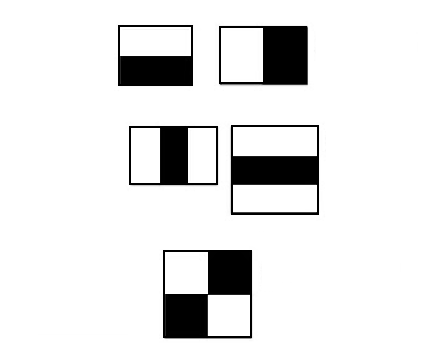
\includegraphics[width=0.6\textwidth]{pic/cechy haara/cechy Haara.png}
	\caption{Cechy Haara pozwalające wykrycie między innymi krawędzi i lini.}
	\label{fig:Cechy-Haara}
\end{figure}








Jeśli „Specyfikacja wewnętrzna”:
\begin{itemize}
\item przedstawienie idei -> wykonanie niezbędnych obliczeń projektowych, syntezy układu
\item architektura systemu -> opis architektury proponowanego rozwiązania
\item opis struktur danych (i organizacji baz danych)
\item komponenty, moduły, biblioteki, przegląd ważniejszych klas (jeśli występują) -> oprogramowania systemu
\item przegląd ważniejszych algorytmów (jeśli występują) !!!
\item szczegóły implementacji wybranych fragmentów, zastosowane wzorce projektowe !!!
\item diagramy UML
\end{itemize}



% % % % % % % % % % % % % % % % % % % % % % % % % % % % % % % % % % % 
% Pakiet minted wymaga importu: \usepackage{minted}                 %
% i specjalnego kompilowania:                                       %
% pdflatex -shell-escape main                                       %
% % % % % % % % % % % % % % % % % % % % % % % % % % % % % % % % % % % 


Krótka wstawka kodu w linii tekstu jest możliwa, np.  \lstinline|int a;| (biblioteka \texttt{listings})% lub  \mintinline{C++}|int a;| (biblioteka \texttt{minted})
. 
Dłuższe fragmenty lepiej jest umieszczać jako rysunek, np. kod na rys \ref{fig:pseudokod:listings}% i rys. \ref{fig:pseudokod:minted}
, a naprawdę długie fragmenty – w załączniku.


\begin{figure}
\centering
\begin{lstlisting}
class test : public basic
{
    public:
      test (int a);
      friend std::ostream operator<<(std::ostream & s, 
                                     const test & t);
    protected:
      int _a;  
      
};
\end{lstlisting}
\caption{Pseudokod w \texttt{listings}.}
\label{fig:pseudokod:listings}
\end{figure}

%\begin{figure}
%\centering
%\begin{minted}[linenos,frame=lines]{c++}
%class test : public basic
%{
%    public:
%      test (int a);
%      friend std::ostream operator<<(std::ostream & s, 
%                                     const test & t);
%    protected:
%      int _a;  
%      
%};
%\end{minted}
%\caption{Pseudokod w \texttt{minted}.}
%\label{fig:pseudokod:minted}
%\end{figure}




%--------------------------------------
%
%
% TODO: sposób testowania w ramach pracy, organizacja eksperymentów, przypadki testowe zakres testowania, wykryte i usunięte błędy, opcjonalnie wyniki badań eksperymentalnych
%
% Status: 0%
%--------------------------------------
\chapter{Weryfikacja i walidacja}
\label{ch:06}
\begin{itemize}
\item sposób testowania w ramach pracy (np. odniesienie do modelu V)
\item organizacja eksperymentów
\item przypadki testowe zakres testowania (pełny/niepełny)
\item wykryte i usunięte błędy
\item opcjonalnie wyniki badań eksperymentalnych
\end{itemize}

\begin{table}
\centering
\caption{Nagłówek tabeli jest nad tabelą.}
\label{id:tab:wyniki}
\begin{tabular}{rrrrrrrr}
\toprule
	         &                                     \multicolumn{7}{c}{metoda}                                      \\
	         \cmidrule{2-8}
	         &         &         &        \multicolumn{3}{c}{alg. 3}        & \multicolumn{2}{c}{alg. 4, $\gamma = 2$} \\
	         \cmidrule(r){4-6}\cmidrule(r){7-8}
	$\zeta$ &     alg. 1 &   alg. 2 & $\alpha= 1.5$ & $\alpha= 2$ & $\alpha= 3$ &   $\beta = 0.1$  &   $\beta = -0.1$ \\
\midrule
	       0 &  8.3250 & 1.45305 &       7.5791 &    14.8517 &    20.0028 & 1.16396 &                       1.1365 \\
	       5 &  0.6111 & 2.27126 &       6.9952 &    13.8560 &    18.6064 & 1.18659 &                       1.1630 \\
	      10 & 11.6126 & 2.69218 &       6.2520 &    12.5202 &    16.8278 & 1.23180 &                       1.2045 \\
	      15 &  0.5665 & 2.95046 &       5.7753 &    11.4588 &    15.4837 & 1.25131 &                       1.2614 \\
	      20 & 15.8728 & 3.07225 &       5.3071 &    10.3935 &    13.8738 & 1.25307 &                       1.2217 \\
	      25 &  0.9791 & 3.19034 &       5.4575 &     9.9533 &    13.0721 & 1.27104 &                       1.2640 \\
	      30 &  2.0228 & 3.27474 &       5.7461 &     9.7164 &    12.2637 & 1.33404 &                       1.3209 \\
	      35 & 13.4210 & 3.36086 &       6.6735 &    10.0442 &    12.0270 & 1.35385 &                       1.3059 \\
	      40 & 13.2226 & 3.36420 &       7.7248 &    10.4495 &    12.0379 & 1.34919 &                       1.2768 \\
	      45 & 12.8445 & 3.47436 &       8.5539 &    10.8552 &    12.2773 & 1.42303 &                       1.4362 \\
	      50 & 12.9245 & 3.58228 &       9.2702 &    11.2183 &    12.3990 & 1.40922 &                       1.3724 \\
\bottomrule
\end{tabular}
\end{table}  



%--------------------------------------
%
%
% TODO: uzyskane wyniki, kierunki ewentualnych dalszych prac, problemy napotkane w trakcie pracy, wnioski
%
% Status: 0%
%--------------------------------------
\chapter{Podsumowanie i wnioski}
\begin{itemize}
\item uzyskane wyniki w świetle postawionych celów i zdefiniowanych wyżej wymagań
\item kierunki ewentualnych danych prac (rozbudowa funkcjonalna …)
\item problemy napotkane w trakcie pracy
\end{itemize}



\backmatter

%\bibliographystyle{plplain}  % bibtex
%\bibliography{biblio} % bibtex
\printbibliography           % biblatex
\addcontentsline{toc}{chapter}{Bibliografia}

\begin{appendices}

%--------------------------------------
%
%
% TODO: skróty z tekstu
%
% Status: ?%
%--------------------------------------
\chapter{Spis skrótów i symboli}

\begin{itemize}
\item[DNA] kwas deoksyrybonukleinowy (ang. \english{deoxyribonucleic acid})
\item[MVC] model -- widok -- kontroler (ang. \english{model--view--controller}) 
\item[$N$] liczebność zbioru danych
\item[$\mu$] stopnień przyleżności do zbioru
\item[$\mathbb{E}$] zbiór krawędzi grafu
\item[$\mathcal{L}$] transformata Laplace'a 
\end{itemize}


%--------------------------------------
%
%
% TODO: długi fragment źródła
%
% Status: ?%
%--------------------------------------
\chapter{Źródła}

Jeżeli w pracy konieczne jest umieszczenie długich fragmentów kodu źródłowego, należy je przenieść w to miejsce.

\begin{lstlisting}
if (_nClusters < 1)
	throw std::string ("unknown number of clusters");
if (_nIterations < 1 and _epsilon < 0)
	throw std::string ("You should set a maximal number of iteration or minimal difference -- epsilon.");
if (_nIterations > 0 and _epsilon > 0)
	throw std::string ("Both number of iterations and minimal epsilon set -- you should set either number of iterations or minimal epsilon.");
\end{lstlisting}


% % % % % % % % % % % % % % % % % % % % % % % % % % % % % % % % % % % 
% Pakiet minted wymaga odkomentowania w pliku config/settings.tex   %
% importu pakietu minted: \usepackage{minted}                       %
% i specjalnego kompilowania:                                       %
% pdflatex -shell-escape praca                                      %
% % % % % % % % % % % % % % % % % % % % % % % % % % % % % % % % % % % 

%\begin{minted}[linenos,breaklines,frame=lines]{c++}
%if (_nClusters < 1)
%   throw std::string ("unknown number of clusters");
%if (_nIterations < 1 and _epsilon < 0)
%   throw std::string ("You should set a maximal number of iteration or minimal difference -- epsilon.");
%if (_nIterations > 0 and _epsilon > 0)
%   throw std::string ("Both number of iterations and minimal epsilon set -- you should set either number of iterations or minimal epsilon.");
%\end{minted}


%--------------------------------------
%
%
% TODO: źródła programu, dane testowe, film pokazujący działanie oprogramowania
%
% Status: 0%
%--------------------------------------
\chapter{Lista dodatkowych plików, uzupełniających tekst pracy} 


W systemie do pracy dołączono dodatkowe pliki zawierające:
\begin{itemize}
\item źródła programu,
\item dane testowe,
\item film pokazujący działanie opracowanego oprogramowania lub zaprojektowanego i~wykonanego urządzenia,
\item itp.
\end{itemize}


\listoffigures
\addcontentsline{toc}{chapter}{Spis rysunków}
\listoftables
\addcontentsline{toc}{chapter}{Spis tabel}

\end{appendices}

\end{document}


%% Finis coronat opus.

